%%%%%%%%%%%%%%%%%%%%%%%%%%%%%%%%%%%%%%%%%
% OIST Doctoral Thesis - Final bound version
% LaTeX Template
% Version 0.2 (2016/04/06)
%
% This version is the final binding version which will be published.
%
% Original author:
% Jeremie Gillet
%
%%%%%%%%%%%%%%%%%%%%%%%%%%%%%%%%%%%%%%%%%

%----------------------------------------------------------------------------------------
%	PACKAGES AND OTHER DOCUMENT CONFIGURATIONS
%----------------------------------------------------------------------------------------

\documentclass[12pt, oneside]{book} % 12 pt font, two-sided book style
\usepackage[a4paper, includehead, headheight=0.6cm, inner=3cm ,outer=2.5cm, top=2.5 cm, bottom=2.5cm]{geometry}  % Changing size of document
\usepackage[english]{babel} % The document is in English
\usepackage[utf8]{inputenc} % UTF8 encoding
\usepackage[T1]{fontenc} % Font encoding

\usepackage{graphicx} % For including images
\graphicspath{{./Figures/}} % Specifies the directory where pictures are stored

\usepackage{longtable} % tables that can span several pages
\usepackage[bf]{caption} % caption: FIG in bold
\usepackage{fancyhdr} % For the headers

\usepackage{titlesec}
\titleformat{\chapter}[hang]
{\normalfont\huge\bfseries}{\thechapter}{20pt}{\Huge}
\titleformat{\section}
{\normalfont\Large\bfseries}{\thesection}{1em}{}

\newcommand{\numberedchapter}{ % Preparation for numbered chapters
%	\cleardoublepage % To make sure the previous headers are passed
	\fancyhead[RE]{{\bfseries \leftmark}}% Headers for left pages
	\fancyhead[LO]{{\bfseries \rightmark}}}% Headers for right pages
\newcommand{\unnumberedchapter}[1]{ % Preparation for unnumbered chapters
%	\cleardoublepage % To make sure the previous headers are passed
	\addcontentsline{toc}{chapter}{#1} % Also adds the chapter name to the Contents
	\fancyhead[RE]{{\bfseries #1}} % Headers for left pages
	\fancyhead[LO]{}}%Headers for right pages

\usepackage{emptypage} % No headers on an empty page

\usepackage{eso-pic} % For the background picture on the title page
\newcommand\BackgroundPic{%
\put(-250,-160){%
\parbox[b][\paperheight]{\paperwidth}{%
\vfill
\centering
\includegraphics[width=\paperwidth]{symbol.jpg}%
\vfill
}}}

\usepackage{hyperref} % Adds clickable links at references

%----------------------------------------------------------------------------------------
%	ADD YOUR CUSTOM VALUES, COMMANDS AND PACKAGES
%----------------------------------------------------------------------------------------

% Open Preamble/mydefinitions.tex and enter some values (name, thesis title...) 
% and include your own custom LaTeX functions and packages

%----------------------------------------------------------------------------------------
%	COMMANDS FOR THE THESIS
%----------------------------------------------------------------------------------------

\newcommand{\name}{Joanna Piper Morgan} % Author name
\newcommand{\thesistitle}{Piper's Ponderings} % Title of the thesis
\newcommand{\submissiondate}{September, 2024} % Submission date "Month, year"
\newcommand{\advisor}{Kyle E. Niemeyer} % Supervisor name
%\newcommand{\coadvisor}{Someone Someone} % Co-Supervisor name, comment this line if there is none


%----------------------------------------------------------------------------------------
%	BIBLIOGRAPHY STYLE (pick the style you want)
%----------------------------------------------------------------------------------------

\usepackage[square, numbers, sort&compress]{natbib} % for bibliography - Square brackets, citing references with numbers, citations sorted by appearance in the text and compressed (as in [4-7])
%\usepackage[longnamesfirst,round]{natbib} % Natural Sciences bibliography

\bibliographystyle{Preamble/physics_bibstyle} % You may use a different style adapted to your field
%\bibliographystyle{unsrtnat} % You may use a different style adapted to your field


%----------------------------------------------------------------------------------------
%	PACKAGES (be careful of package interaction)
%----------------------------------------------------------------------------------------

\usepackage{amsmath, amsthm, amssymb, amsfonts, amstext, bm, bbm, mathtools} % Math symbols
\usepackage{graphicx, subfigure, caption, epsfig, psfrag} % Figures
\usepackage{threeparttable, colortbl, multirow} % Tables
\usepackage{soul, pifont, color, hyperref, bbding, textcomp, manfnt, latexsym, wasysym} % Fonts
\usepackage{enumitem}
\usepackage[ruled, vlined]{algorithm2e}
% \usepackage[makeroom]{cancel}
\usepackage{lscape}
\usepackage{pdfpages}

%----------------------------------------------------------------------------------------
%	DEFINITIONS AND COMMANDS
%----------------------------------------------------------------------------------------

% Defining a theorem box for Criteria
\newtheorem{critere}{Criterion}
\newcommand{\crit}[2]{
\begin{center}  
\fbox{ \begin{minipage}[c]{0.9 \textwidth}
\begin{critere}
\textbf{\textup{ #1}} --- #2
\end{critere}
\end{minipage}  } \end{center}
}

\newcommand{\todo}[1]{\textcolor{red}{(#1)}}
% todo command from https://tex.stackexchange.com/questions/247681/how-to-create-checkbox-todo-list
\usepackage{enumitem}
\newlist{todolist}{itemize}{2}
\setlist[todolist]{label=$\square$}
% \usepackage{pifont}
\newcommand{\cmark}{\ding{51}}
\newcommand{\xmark}{\ding{55}}
\newcommand{\done}{\rlap{$\square$}{\raisebox{2pt}%
{\large\hspace{1pt}\cmark}}\hspace{-2.5pt}}
\newcommand{\cancel}{\rlap{$\square$}{\large\hspace{1pt}\xmark}}

\newcommand{\eg}{\textit{e.g.}}
\newcommand{\ie}{\textit{i.e.}}

% General
\newcommand{\bea}{\begin{eqnarray}} % Shortcut for equation arrays
\newcommand{\eea}{\end{eqnarray}}
\newcommand{\defin}{\triangleq}
\newcommand{\pdiff}[2]{ \frac{ \partial #1 }{ \partial #2 } }
\newcommand{\red}[1]{{\color{red}\textbf{#1}}}
\newcommand{\blue}[1]{{\color{blue} #1}}
\newcommand{\green}[1]{{\color{ForestGreen}\textbf{#1}}}
\newcommand{\tal}[1]{\textbf{\alert{#1}}}

% Attenuation equation
\newcommand{\StmD}{\Sigma_t^\Delta \Delta x}
\newcommand{\StdD}{\Sigma_t^\Delta \Delta x}
\newcommand{\Stm}{\Sigma_{t,m}^{0}}
\newcommand{\Std}{\Sigma_{t,m}^{\Delta}}

% Var and EE
\newcommand{\Var}[1]{\mathbb{V}ar\left[#1\right]}
\newcommand{\EE}[1]{\mathbb{E}\left[#1\right]}
\newcommand{\Cov}[2]{\mathbb{C}ov\left[#1,#2\right]}

% Xi
\newcommand{\EExi}[1]{\mathbb{E}_\xi\left[#1\right]}
\newcommand{\Vxi}[1]{\mathbb{V}ar_\xi\left[#1\right]}
\newcommand{\Nxi}{{N_\xi}}
\newcommand{\xii}{\xi^{(i)}}
\newcommand{\sumxi}{\sum_{i=1}^{\Nxi}}

% Eta
\newcommand{\EEeta}[1]{\mathbb{E}_\eta\left[#1\right]}
\newcommand{\Veta}[1]{\mathbb{V}ar_\eta\left[#1\right]}
\newcommand{\Neta}{{N_\eta}}
\newcommand{\etaj}{\eta^{(j)}}
\newcommand{\etak}{\eta^{(k)}}
\newcommand{\Zeta}{ {Z_\eta} }
\newcommand{\muRT}{\hat{\mu}_{\SigSqRT}}
\newcommand{\sumeta}{\sum_{j=1}^\Neta}

% Estimators
\newcommand{\Qpoll}{\tilde{Q}}
\newcommand{\Qhat}{\hat{Q}}
\newcommand{\SigSqeta}{\sigma^2_\eta}
\newcommand{\SigSqRT}{\sigma^2_{RT,\Neta}}
\newcommand{\hatSigSqeta}{\hat{\sigma}^2_\eta}
\newcommand{\fij}{f(\xii,\etaj)}
\newcommand{\f}{f(\xi,\eta)}
\newcommand{\ft}{\tilde{f}}

% Omega
\newcommand{\EEom}[1]{\mathbb{E}_\omega\left[#1\right]}
\newcommand{\Vom}[1]{\mathbb{V}ar_\omega\left[#1\right]}
\newcommand{\Nom}{{N_\omega}}
\newcommand{\EExo}[1]{\mathbb{E}_{\xi,\omega}\left[#1\right]}
\newcommand{\Vxo}[1]{\mathbb{V}ar_{\xi,\omega}\left[#1\right]}
\newcommand{\Qxo}{Q\left(\xi,\omega\right)}
\newcommand{\PE}{ {\mathbb{P}_{\mathbb{E}}} }
\newcommand{\Pxi}{ \mathbb{P}_{\mathbb{E | \xi}} }
\newcommand{\PEpollom}{ \tilde{\mathbb{P}}^{\mathbb{E}}_{\Nom} }

% SM Example problem
\newcommand{\T}[1][]{T^{#1}\left( \xi, \omega \right)}
\newcommand{\PA}{p_1}
\newcommand{\SA}{\Sigma_{t,1}}
\newcommand{\SB}{\Sigma_{t,2}}
\newcommand{\SC}{\Sigma_{t,3}}
\newcommand{\StC}{\Sigma_{t,3}^{0}}
\newcommand{\StCd}{\Sigma_{t,3}^{\Delta}}
\newcommand{\Dx}{ \Delta x}
\newcommand{\DxA}{ \Delta x_A}
\newcommand{\DxB}{ \Delta x_B}
\newcommand{\Nt}{N_{tot}}
\newcommand{\NA}{N_1(\omega)}
\newcommand{\FAB}{F(\xi_A,\xi_B)}
\newcommand{\Fm}{F_0}
\newcommand{\Fd}{F_{\Delta}(\xi_A,\xi_B)}
\newcommand{\xiA}{\xi_A}
\newcommand{\xiB}{\xi_B}
\newcommand{\Bom}{B_\omega(x)}
\newcommand{\Bomy}{B_\omega(y)}
\newcommand{\intsin}[1]{\frac{ \sinh\left[ #1 \right] }{ #1 }}
\newcommand{\e}[1]{\exp \left( #1 \right) }
\newcommand{\sinhh}[1]{\text{sinh}\left[ #1 \right]}
\newcommand{\g}{\, | \,}


% PCE
\newcommand{\xiu}{{\xi_u}}
\newcommand{\xinu}{{\xi_{\sim u}}}
\newcommand{\Nsi}{{N_{SI}}}
\newcommand{\EEu}[1]{\mathbb{E}_{\xiu} \left[#1\right]}
\newcommand{\EEnu}[1]{\mathbb{E}_{\xinu} \left[#1\right]}
\newcommand{\Vu}[1]{\mathbb{V}ar_{\xiu}\left[#1\right]}
\newcommand{\Vnu}[1]{\mathbb{V}ar_{\xinu} \left[#1\right]}
\newcommand{\Ppoll}{\tilde{P}_\Nsi}
\newcommand{\hf}{\mathrm{HF}}
\newcommand{\LF}{\mathrm{LF}}
\newcommand{\kn}{{\Large\dbend\normalsize\hspace{1mm}}}
\newcommand{\PCE}{Q^{PC}}
\newcommand{\PCvar}{\hat{\sigma}^{2}_{PC}}



\begin{document}

%----------------------------------------------------------------------------------------
%	TITLE PAGE
%----------------------------------------------------------------------------------------

\pagestyle{empty} % No page numbers
\frontmatter % Use roman page numbering style (i, ii, iii, iv...) for the preamble pages

\begin{titlepage}
%\AddToShipoutPicture*{\BackgroundPic}
\begin{center}
\vfill
{\large \scshape School of Mechanical, Industrial and Manufacturing Engineering \\Oregon State University}\\[1.4cm]
{\Large PhD Thesis Proposal}\\[1.4cm]
%\rule{\textwidth}{1.5pt}\\[0cm]
{\huge \bfseries \thesistitle \par \ }\\[-0.5cm]
%\rule{\textwidth}{1.5pt}\\[2.5cm]
\hfill  \\[1cm]
\hfill  {\large \bfseries\name}\\
\vfill
{\hfill \large Advisor: \textbf{\advisor}} \\ 
\ifx\coadvisor\undefined\else{\hfill \large Co-Advisor: \textbf{\coadvisor}} \\ \fi
\vspace{1cm}
\hfill  \submissiondate
\end{center}
\end{titlepage}

%----------------------------------------------------------------------------------------
%	PREAMBLE PAGES (comment out unnecessary pages)
%----------------------------------------------------------------------------------------

\pagestyle{fancy} % Changes the headers
\renewcommand{\chaptermark}[1]{ \markboth{#1}{}} % Getting the chapter name right
\renewcommand{\sectionmark}[1]{\markright{\thesection\; #1}} % Getting the section name right
\fancyhf{}% Clears header and footer
\fancyhead[RO,L]{\thepage} % page number on the outside of headers

% \unnumberedchapter{Abstract} 
\chapter*{Abstract} 
\subsection*{\thesistitle}

This should be a single paragraph of not more than 500 words, which concisely summarizes the entire proposal.

%----------------------------------------------------------------------------------------
%	LIST OF CONTENTS/FIGURES/TABLES
%----------------------------------------------------------------------------------------

\unnumberedchapter{Contents}
\tableofcontents % Write out the Table of Contents

%----------------------------------------------------------------------------------------
%	THESIS MAIN TEXT - CHAPTERS
%----------------------------------------------------------------------------------------

% \addtocontents{toc}{\vspace{2em}} % Add a gap in the Contents, for aesthetics
\mainmatter % Begin numeric (1,2,3...) page numbering

\numberedchapter
\chapter{Introduction and background}
\label{ch-intro}

\section {A brief overview}
Predicting how neutral particle radiation moves through space and time is important when modeling inertial confinement fusion systems, pulsed neutron sources, and nuclear criticality safety experiments, among other systems.
Simulating these problems is computationally difficult using any numerical method, as the neutron distribution is a function of seven independent variables: three in space, three in velocity, and time.
% This problem demands HPCs and specifically the exascale
Modern HPC systems now enable high-fidelity simulation of neutron transport for problem types that have seldom been modeled before due to limitations of previous computers. % need citation?
Exploration of both novel numerical methods that can better take advantage of modern HPCs and the methods of implementing them in code are warranted.
% Specifically, large scale, highly dynamic transport problems require thousands of compute nodes using modern hardware accelerators (i.e., GPUs) \cite{hamilton_continuous-energy_2019, romano_openmc_nodate}.

My research is broad in its application but thematically specific, to satiate the ever-present need to go faster: faster and more accurate numerical methods, and faster implementations of numerical methods into HPC-worthy code.
I will first present my research questions, then provide more introduction to demonstrate the gaps in knowledge they seek to probe.
Then I will present my itemized research objectives and tasks required to implement those objectives.
I will briefly describe the methods already implemented and more thoroughly describe methods yet to be done.
Finally I will present preliminary results and draw initial conclusions.

This proposal is heavily supplemented by publications included as appendices.
Explanations of methods and results is intentionally terse as to respect my committees' already generous time commitment and service.
On that note I extend my most heart-felt gratitude to you and am keen and eager for the lively conversations sure to ensue about the work that I love.

\hfill

with mutual respect,

Joanna Piper Morgan

\subsection{Research questions}
\begin{enumerate}
    \item Can relying on abstraction through using software libraries enable non-expert users to produce efficient-performing software for heterogeneous computing systems?
    \item Will a space-parallel deterministic iterative solution algorithm outperform the standard angle-parallel iterative algorithm on heterogeneous architectures?
    \item For deterministic neutron transport, does accounting for transient effects alter convergence rates of the iterative solution algorithms?
    \item Can information coming from a streaming-only problem be used to inform cell boundary information and increase convergence rates of a one-cell inversion iteration algorithm?
    \item How can alternative Monte Carlo tracking schemes (namely Woodcock or delta tracking) be used be used to converge the quantities of interest faster?
\end{enumerate}

% Some already answered MC question
% phrase as hypthisys or hyp to q

\section{Neutron transport}

Transport equations are, at their most fundamental,equations of continuity.
Due to their ubiquity in nature, transport equations are used to describe an incredible number of physical systems including fluid dynamics, chemical reactions, electromagnetism, energy, and heat transfer.
My research contained herein focuses on neutron radiation transport specifically, but could easily be applied to other neutral particles, most relevantly photons \cite{radheattrans2003, chandrasekhar1960radiative}.
In fact many of the methods of solution described in this document started as approximations for radiative heat transfer or photon transport.
%justifying my ME degree
Assuming no neutrons are being produced by fission, the neutron transport equation (NTE) takes the form of an intergro-partial differential Boltzmann-type equation with seven independent variables \cite{duderstadt_hamilton}.
As with any other continuity equation it is written as a set of sources (on the right) and sinks (on the left):
\begin{multline}
    \label{eq:fullNTE}
    \frac{1}{v(E)}\frac{\partial \psi(\boldsymbol{r}, E, \boldsymbol{\hat{\Omega}},t)}{\partial t} + \boldsymbol{\hat{\Omega}} \cdot \nabla \psi(\boldsymbol{r}, E, \boldsymbol{\hat{\Omega}},t) + \Sigma(r, E, t) \psi(\boldsymbol{r}, E, \boldsymbol{\hat{\Omega}},t) = \\
    \int_{4\pi}\int_{0}^{\infty}\Sigma_s(\boldsymbol{r}, E'\rightarrow E, \boldsymbol{\hat{\Omega}'} \rightarrow \boldsymbol{\hat{\Omega}}, t)
    \psi(\boldsymbol{r}, E, \boldsymbol{\hat{\Omega}},t) dE' d\boldsymbol{\hat{\Omega}'} +
    s(\boldsymbol{r}, E, \boldsymbol{\hat{\Omega}},t) \;,
\end{multline}
where $\psi$ is the angular flux, $v$ is the velocity of the particles, $\Sigma$ is the macroscopic total material cross section, $\Sigma_s$ is the macroscopic scattering cross section, $\boldsymbol{r}$ is the location of the particle in three-dimensional space, $\boldsymbol{\hat{\Omega}}$ is the direction of travel in three-dimensional space, $s$ is the source of new particles being produced, $t$ is the time, and $E$ is the energy of the particles for $\boldsymbol{r} \in V$, $\boldsymbol{\hat{\Omega}} \in 4\pi$, $0<E<\infty$, and $0<t$ \cite{duderstadt_hamilton}. We also prescribe the initial condition
\begin{equation}
    \psi(\boldsymbol{r}, E, \boldsymbol{\hat{\Omega}},0) = \psi_{initial}(\boldsymbol{r}, E, \boldsymbol{\hat{\Omega}})
\end{equation}
and the boundary condition
\begin{equation}
    \psi(\boldsymbol{r}, E, \boldsymbol{\hat{\Omega}},t) = \psi_{bound}(\boldsymbol{r}, E, \boldsymbol{\hat{\Omega}},t) \text{ for } \boldsymbol{r} \in \partial V \text{ and } \boldsymbol{\hat{\Omega}} \cdot \boldsymbol{n} < 0 \;.
\end{equation}
A number of additional implicit assumptions are needed for the validity of this equation and my research including: particle-particle interactions are rare and can be neglected, neutrons are points in space with no volume, collision events occur instantaneously, and nuclear properties are known \cite{lewis_computational_1984}.
This equation is commonly solved using both deterministic and Monte Carlo solution methods as analytic solutions are sparse.

\section{Deterministic methods}

To recast the neutron radiation transport equation (eq \ref{eq:fullNTE}) into a form solvable on digital computers continuous functions of space, time, angle, and energy must be discretized.
Due to the nature of the NTE (intergro-PDEy-ness) an iterative scheme is also required.
In this section I describe the discretizations and their assumptions for the 1D, time-dependent, multi-group solver proposed within this work.
I will also describe the two fixed-point iterative schemes that I implement and discuss gaps in previous work of deterministic iterative solvers.
My work with deterministic schemes can be separated into two categories:
\begin{enumerate}
    \item How to use software engineering libraries to implement work more efficiently (RQ 1); and
    \item Considering novel methods to converge the solution faster on modern hardware
    \begin{enumerate}
        \item A space-parallel iterative scheme on modern HPC GPUs (RQ2);
        \item How transient behavior impacts convergence of a space-parallel iterative scheme (RQ3); and
        \item How to accelerate the space-parallel iterative scheme to converge faster (RQ4)
    \end{enumerate}
\end{enumerate}

\subsection{S$_N$ approximation in angle}

The S$_N$ or discrete ordinance approximation turns the introgro-PDE describing radiation transport into a coupled (simultaneous) set of linear PDEs in each angular direction.
It was first formulated by Chandrasekhar to describe radiative heat transfer in stellar media \cite{chandrasekhar1960radiative}.
The S$_N$ approximation was soon applied to neutron transport by Carlson \cite{precise1971carlson}, Lee \cite{discrete1961lee}, and Lathrop \cite{discrete1966lathnrop}.
The method of discrete ordinance was also adapted to general radiative heat transfer by Fiveland \cite{three1988fiveland} and Truelove \cite{discrete1987truelove}.
%While this work is only concerned with the S$_N$ approximations another approximation using the method of moments and orthogonal spherical harmonics as basis functions can also be used to approximate the angular integral which gives rise to the P$_N$ approximations \cite{radheattrans1990}.

At this point it becomes necessary to describe the other governing assumptions I use in this work including:
slab geometry (1D-rectilinear coordinates), isotropic scattering and sources, as well as the multi-group assumption in energy distribution.
The methods I propose in this work are not restricted by these assumptions---and future work may extend the methods described herein to be valid for anisotropic distributions in angle and/or solutions on unstructured meshes----but are made here for simplicity.
In-fact I make specific decisions in this work with the underlying discretization schemes to allow for eventual extension to these regimes.

When applied to equation \ref{eq:fullNTE} the resulting initialization point for my work is described by
\begin{multline}
    \label{eq:sn_nte}
    \frac{1}{v_g} \frac{\partial \psi_{m,g}(x,t)}{\partial t} + \mu_m \frac{\partial \psi_{m,g}(x,t)}{\partial x} + \Sigma_g(x) \psi_{m,g}(x,t)  \\
     = \frac{1}{2} \left( \sum\limits_{g' = 0}^G \Sigma_{s, g'\to g}(x) \sum\limits_{n=1}^N w_n \psi_{n, g'}(x,t) + Q_g(x,t) \right) \;, \\
    \qquad g=1 \ldots G \;, \qquad m=1 \ldots N \;, \qquad t > 0 \;, \qquad x \in [0,X] \;,
\end{multline}
where $\psi$ is the angular flux, $t$ is time, $x$ is location in 1D space, $g$ refers to the group, $v$ is velocity, $w_m$ is angular quadrature weight, $\mu_m$ is the angular quadrature ordinate ($\cos(\hat{\Omega}_\theta)$), $m$ is the quadrature index, and $Q$ is the isotropic material source.
In this work I will exclusively use Gauss-Legendre quadrature, but if extended to higher dimensions other quadratures sets would be required to evaluate the double integral over both angular directions (e.g. level-symmetric). 
The initial and boundary conditions are again prescribed angular flux distributions:
\begin{equation*}
    \psi_{m,g}(x,0) = \psi_{m,0}(x), \qquad m=1 \ldots N \;,
\end{equation*}
\begin{equation*}
    \psi_{m,g}(0,t) = \psi_{m,L}(t), \qquad \mu_m >0 \;,
\end{equation*}
\begin{equation*}
    \psi_{m,g}(X,t) = \psi_{m,R}(t), \qquad \mu_m <0 \;.
\end{equation*}
From here additional discretization can be used to turn the continuous functions of angular flux, source, material data, and differential operators into numerical approximations.

\subsection{Time-Space discretization schemes}

To enable this work in both space and time, discretization schemes are needed to treat the differential operators and continuous functions.
As the goal of the research is for development on heterogeneous architectures communication to work ratio may become an issue.
Numerical algorithms that require lots of communication back and forth between the host (CPU) and device (GPU) will limit the maximum allowable performance for most GPU accelerators.
To abate this issue higher (second) order discretization schemes can be used to add to the compute work required in every iteration, thus improving the communication to work ratio.

Various classes of spatial discretizations can be used in radiation transport.
Finite difference, finite element, and finite volume methods are all often employed with the most common scheme being Diamond-Differencing $\mathcal{O}(2)$.
Diamond-Difference is popular as it is the only second order space discretization that uses a single interior (cell-averaged) degree of freedom; however it only works on orthogonal grids.
%Intended future investigation of the scheme in this research are into non-uniform meshes.
While I will not include that analysis in this work, I do want to leave that opportunity open in order to better mesh with the modern state of the art of transport solvers which is on unstructured girds.
Therefore, I used a finite volume scheme specifically designed for use on unstructured grids called corner-balance, which was originally developed by Adams~\cite{adams_subcell_1997}.
It is a finite volume method and enforces conservation within subcell volumes in a spatial cell.
Simple corner balance was determined to be sufficient as it is higher $\mathcal{O}(2)$ order.
%Simple corner blance is not acrurate in the thin-limit however a slight alteration to it 
In 1-D slab geometry, simple corner balance is equivalent to the lumped-linear discontinuous finite element method.

Solving the transport equation with deterministic methods typically involves iterative schemes to converge the scattering source and transport operators (this is discussed more in section \ref{sec:intro_itterative-scheme}).
Thus implicit time marching schemes are often used to time step as they have desirable stability properties.
Specifically, implicit (backward) Euler $\mathcal{O}(1)$ or Crank-Nicolson $\mathcal{O}(2)$ are the most often employed.
%These schemes are advantageous as they often act like a wrapper around a steady state deterministic transport solver with few changes needed to implement.
While Crank-Nicolson is second order accurate it is not robust and can produce negative solutions and spurious osculations.
Time dependent multiple balance (TDMB) was derived by Variansyah, Larsen, and Martin~\cite{variansyah_robust_2021} to be a robust higher (second) order time discretization scheme.
TDMB is developed from the physics informed "multiple-balance" approach which has also been developed as a space discretization scheme.
When implementing a higher order method to allow for greater work-to-communicate ratios I decided to use this scheme. 

\subsection{Source-iteration}
\label{sec:intro_itterative-scheme}

The transport equation requires some kind of iterative scheme to converge the linkage between scattering source and transport operators.
The source iteration (SI) method is commonly used to do this, often accompanied by preconditioners or synthetic accelerators, where the contribution to the solution from the scattering source (summation in the RHS of equation \ref{eq:sn_nte}) is allowed to lag, while the angular flux is solved in every ordinate via transport sweeps through the spatial domain \cite{adams_subcell_1997}.
SI sweeps in Cartesian geometries are readily parallelized over the number of angles, as the source term is known from the previous iteration, allowing the angular flux in each ordinate to be computed independently. 
While any parallelization is a boon to performance, a scheme that is embarrassingly parallel over the dimension with the greatest number of degrees of freedom---space---may be advantageous.
In a single spatial dimension SI is \textit{annoying serial} in space and cannot be parallelized.

In higher spatial dimensions, many S$_N$ production codes that implement SI use some kind of wavefront marching parallel algorithm also known as a Kockh-Baker-Alcouff scheme \citep{KBA} also called "full parallel sweeps" in literature.
In this scheme a sweep begins in a spatial location where all cell dependencies are known from boundary information (e.g. a corner).
From there on a hypothetical 2D grid, the two nearest neighbor cells are computed independently, potentially in parallel; the next step would be 4 cells.
This diagonally expanding wavefront continues to march and is able to better parallelize as many cells spatially as possible eventually saturating the number of work threads if the problem is large enough.
%On CPUs this has been shown to be performant but this changing amount of work is not optimal on GPUs where.
%Performance evaluations of production codes that implement KBA on GPUs is sparse in literature and when avaliable is from proxy-apps.
%Ardra has such a proxy app 
%KBA algorithms are also tricky to efficiently implement in domain decomposed where wave front propagation between boundaries can be tricky.
%While this work is concerned with 1 spatial dimension when analyzing the state of the art it is important to consider that this is done.

%This has proven successful in modern transport applications on CPUs 
%(e.g., PARTISN, which implements the Koch--Baker--Alcouffe or KBA algorithm). 
%The state of the art in deterministic S$_N$ radiation transport is multi-group in energy distribution, diamond differencing first order space discretizations or other FEM FVM schemes on unstructured meshes, backward euler time stepping, domain decomposition via parallel block Jacobi, wave front marching schemes like KBA in higher spatial dimensions within a subdomain, and source iterations with diffusion synthetic acceleration (DSA) and potentially accompanied by GMRES solvers. Some examples of production codes that implement this are Partisn, Ardra, Minerate, Capsaicin, Denovo, Silver Fir, etc.
%Here again this is included as a
%Each one of these points becomes more difficult to implement due to angle-parallel SI with KBA, for example domain decomposition 

%Published literature on what schemes are implemented, how and their performance on GPU accelerators is sparse.
%Most of my understanding of what is currently used comes from conversations held at conferences with the developers of the codes themselves.
%One place I was able to find performance data on is a mini-app called Kripky \citep{kunen_kripke_2015}.
%Kripke is the publicly distributed version of Ardra that has performance data available.
%Roofline anylisys of Kripke has been published for performance on an AMD MI200 GPUs \citep{wolfe2022roofline}. 
%Specific k
%We conject that this is due to the nonlinear work load a wavefront marching schemes incurred. 


\subsection{One cell inversion-iteration}

% Intro to OCI and previous work including warsaw 

One Cell Inversions (OCI) (also called cell-wise parallel block Jacobi) is an alternative to SI where all angular fluxes in all ordinates and groups within a cell are computed in a single linear algebra step.
It assumes that the angular fluxes incident on the surfaces of the cell are known from a previous iteration.
OCI allows for parallelizing over the number of cells as each cell is solved independently of the others in a parallel.

Rosa Warsaw and Perks (2013) \cite{rosa_cellwise_2013} previously investigated OCI as a potentially superior iterative scheme over SI on vectroized heterogeneous architectures.
They supposed that because of the parallelism over the dominant domain, inherit data locality, ability to take advantage of LAPACK type libraries, and highly floppy operations present in an OCI type algorithm, it might out-perform an SI based implementation in wall clock runtime.
The study was conducted on state of the art (at the) time RoadRunner super computer at Los Alamos National Lab and took advantage of its 64 bit PowerXCell vectorized accelerator---a precursor to GPGPUs seen in HPCs today.
Rosa et al. implemented OCI in a 2D, multi-group, steady state, code using first order diamond differencing to discretize space, a multi-group scheme in energy distribution, and parallel block Jacobi and Gauss-Sidle iterations.

The authors concluded that the acceleration seen per-iteration in OCI was not enough to make up for the decay in convergence rate that OCI incurs.
As there is no communication of information between cells within an iteration (sometimes called a-synchronicity), OCI can require more iterations to converge to a solution for some of problems. 
Specifically, as cellular optical thickness goes down, OCI's relative performance degrades with a spectral radius not bounded by one independent of scattering ratio.
Figure~\ref{fig:specrad} illustrates this behavior, showing the spectral radii of the two iteration schemes as a function of cell thickness (in mean free path) and the scattering ratio.
These values were computed numerically from an infinite medium problem (via reflecting boundaries) using steady-state calculations in S$_4$. 
The smaller the spectral radius, the faster a method is converging.
The spectral radius for SI depends linearly on the scattering ratio, and for problems that are many mean free paths in size, it is nearly independent of cell optical thickness. 
The spectral radius of OCI decreases substantially as the optical thickness of the cells increases.
\begin{figure}[!htb]
    \centering
    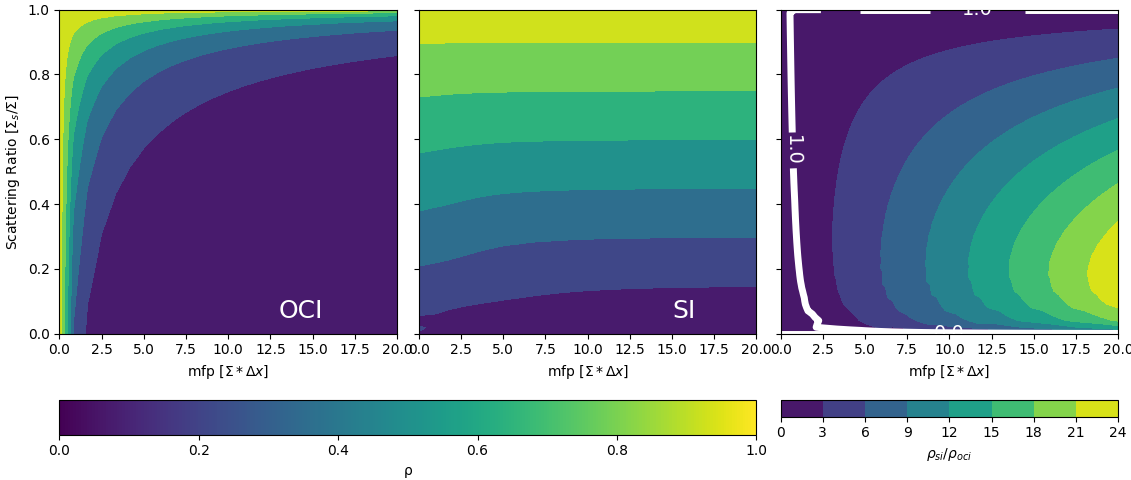
\includegraphics[width=(.9\textwidth)]{figures/spec_rad.png}
    \caption{Spectral radii ($\boldsymbol{\rho}$) of OCI (left) and SI (middle) and the ratio between the two (right), where $\boldsymbol{\Sigma}$ is the total cross section, $\boldsymbol{\Delta x}$ is the cell width, and $\boldsymbol{\Sigma_s}$ is the scattering cross section}
    \label{fig:specrad}
  \end{figure}
Rosa et al. also suggested that future developments in GPGPU accelerators might overcome this convergence rate decay for problems of interest.
The idea there as that even though more iterations will be required to converge a solution those iterations will be able to be done sufficiently faster (in wall-clock-runtime) to mean a solution is computed faster (again in wall clock runtime) then source iterations.

Other investigations have explored OCI as an acceleration scheme for SI \cite{anistratov_iterative_2015, hoagland_hybrid_2021}. %and a solution to the integral transport matrix method \citep{raffi2108pidotscom} and in the inexact parallel Jacobi scheme.
Previous investigations of OCI as an iterative scheme have been limited to steady state computations.

% potential transient effects in the thin limit 
%When solving discrete ordnance problems for transient systems many codes have implemented Crank-Nicholson or backward Euler time stepping.
%These schemes are non-intrusive often looking like an additional time marching loop around the already implemented transport infrastructure.
Regardless of the time stepping method an OCI iterative algorithm might come with some added befits when used in a transient scheme.
Returning to OCI's spectral radius shown at left in Fig.~\ref{fig:specrad}, since both dimensions are governed by relationships with the cross section of the cell ($\Sigma$), altering that value will impact convergence behavior. 
As the scattering ratio decreases, both iterative algorithms require fewer iterations to converge.
However, the spectral radius of OCI also decreases with increasing optical thickness, \textit{which is an added benefit}.
When solving optically thick and highly scattering problems, small increases in $\Sigma$ may drastically improve the relative performance of OCI in comparison with SI.
%Physically this can be understood as single particles living in single cells for many more iterations.
Time step and cellular optical thickness are inversely proportional to each other, meaning a smaller time step will yield a larger effective total cross section, thus theoretically improving the spectral radius.
This behavior is not expected to happen in source iterations as SI does not directly depend on cellular optical thickness---behaving linearly in that dimension for all but the most thick problems.

\subsection{Synthetic acceleration}
% acceleration schemes for SI
In order to converge iterative schemes faster many synthetic acceleration techniques have been explored and implemented over the years \cite{adams_fast_2002}.
The most common used in conjunction with source iterations is diffusion synthetic acceleration (DSA) which converges the slowest mode of SI---the so called diffusive-limit \cite{adams_fast_2002}.
The failure of SI in the diffusive limit can be physically understood as there is no linking between angles within an iteration and a diffusive problem is a coupling of angles.
DSA adds a mid-step correction term based off of a cheap to compute diffusion approximation of transport effects.
Other synthetic acceleration techniques include quasi-diffusion and Boundary projection acceleration \cite{adams_fast_2002}.

% acceleration schemes for OCI
Much less work has gone into exploring synthetic acceleration techniques for one cell inversions.
The slowest mode of convergence of OCI is known to be the thin limit due to the a-synchronicity of the scheme (lagging cell-wise boundary fluxes) \cite{hoagland_hybrid_2021}.
The spectral radius will decay unbounded in the thin limit, regardless of scattering ratio \cite{rosa_cellwise_2013}.
Rosa and Warsa (2009) investigated using transport synthetic acceleration (TSA) as the low order synthetic accelerator via fourier analysis \cite{tsa2009rosa, tsa_slab2006rosa, tsa_2d2007rosa}.
TSA uses a low order transport sweep with potentially fewer angles (when accompanied by SI) and a smaller scattering ratio (often controlled by the user by term $\beta \in [0,1]$) to inform the error correction equation \cite{tsa1997gilles}.
In effect TSA is just a less expensive transport sweep, but a transport sweep none-the-less and comes with all the baggage I am trying to avoid of a transport sweep.
Rosa and Warsa say as much when they suggest a scheme where TSA is only "turned on" after a given number of iterations fails to converge to a solution \cite{tsa2009rosa}.
%TSA
%While they suggest future work to implement, no published results of an OCI+TSA scheme.

% gmres
Both SI and OCI are forms of a fixed-point (or Richardson) iteration that use different operator splittings.
In a fixed-point iteration an initial guess of the angular or scalar flux is supplied as a known to the solver which in turn returns an angular or scalar flux.
This becomes the new guess and is iterated until the relative error between the guess and the output falls to below a given tolerance \cite{lewis1984computational}.
Kyrlov methods on the other hand store multiple copies of the ``guess" as to compute the next guess in a way that is orthogonal of the previous \cite{gmres1996kelley, patton_application_2002}.
Generalized minimal residual method (GMRES) specifically, has been shown to make DSA schemes that preform relatively poorly, work well \cite{kylov2004warsa}.
%They work by keeping copies of the guess for a given number of previous iterates, compute residuals and ensure the next guess is orthogonal to the previous ones\cite{subspace2004warsa}.

\subsection{Novelty and relation to research questions}

The hypothesized additional benefit of of OCI in a time dependent code (RQ 3) coupled with the vast improvements in GPGPU accelerators in the past decade since Rosa et al. \cite{rosa_cellwise_2013} conducted their investigations (RQ 1 and 2), along with the ability to explore higher order spatial and transient discretization schemes (RQ 2) motivates the first publication associated with this work.
After that an exploration of a synthetic acceleration algorithm to converge OCI in the thin limit will become the second (RQ 4).
%Furthermore, as previously mentioned, source iterations are often implemented in production accompanied by some kind of synthetic-acceleration scheme or other preconditioner to converge it's slowest converging mode (the diffusive limit).
%OCI has never been implemented with a prevonditon

\section {Monte Carlo methods}

%Predicting how neutrons move through space and time is important when modeling inertial confinement fusion systems, pulsed neutron sources, and nuclear criticality safety experiments, among other systems.

While deterministic schemes produce an exact solution to an inexact problem Monte Carlo methods provide an inexact solution---with an associated error---to an exact problem.
Monte Carlo methods can treat the independent variables of the NTE (space, angle, time, energy) as continuous, thus eliminating the discretization errors seen with deterministic methods.
The behavior of neutrons can be modeled with a Monte Carlo simulation, where pseudo-particles with statistical importance are created and transported to produce a particle history \cite{lewis_computational_1984}.
A particle's path and the specific set of events that occur within its history are governed by pseudo-random numbers, known probabilities (e.g., from material data), and known geometries.
Data about how particles move and/or interact with the system are tallied to solve for parameters of interest with an associated statistical error from the Monte Carlo process. 
The analog Monte Carlo method is slow to converge (with a convergence rate of $\mathcal{O}(1/\sqrt{n})$ where $n$ is the number of simulated particles).
New Monte Carlo schemes could converge the solution faster in wall-clock time with fewer simulated particles and may be needed to effectively simulate some systems.

%history with interesting citations
%Monte Carlo methods where orignal propased by Stanislaw Ulam in 1946 after work on the Manhattan project.
%It's orginal use in fact was the tracking neutrons thru phase space using handheld computers called Fermiacs.
%The challenge problem I seek to investate also dates back this time.
%Since then from a report in 1995 over 60\% of computational time on US Government super computing systems was concerend with converging the Monte Carlo method

% deception of the section
My work with Monte Carlo schemes---as with my deterministic work---is broadly divided into two categories
\begin{enumerate}
    \item How to use software engineering libraries to implement work more efficiently (RQ 1); and
    \item Considering novel methods to converge the solution faster on modern hardware (RQ 5).
\end{enumerate}
The first section digs into the first goal examining performance portability schemes in high level languages and the work that is currently deployed in Monte Carlo/Dynamic Code (MC/DC) as part of my work with the Center for Exascale Monte Carlo Neutron Transport (CEMeNT).
The second contains work initially done in a production code at Los Alamos National Laboratory and a proposed extension of the scheme the scheme in an implementation in MC/DC.

\subsection{Portability frameworks for Monte Carlo methods}

In this section I introduce initial investigations into high-level performance portability frameworks and discuss 
Developing software to simulate physical problems that demand high-performance computing (HPC) is difficult.
Modern HPCs commonly use both CPUs and GPUs from various vendors.
Years can be spent porting a code from CPUs to run on GPUs, then again when moving from one GPU vendor to the next \cite{pozulp_progress_2023}.
Portability issues compound when designing software for rapidly developing numerical methods where algorithms need to be both implemented and tested at scale.
Finding a software engineering approach that balances the need for portability, rapid development, open collaboration, and performance can be challenging especially when numerical schemes do not rely on commonly library implemented operations (i.e., linear algebra as in LAPACK or Intel MKL). 
% one paragraph for CISE reqirments

Common HPC software engineering requirements are often met using a Python-as-glue-based approach, where peripheral functionality (e.g., MPI calls, I/O) is implemented using Python packages but compiled functions are called through Python's C-interface where performance is needed.
Python-as-glue does not necessarily assist in the production of the compiled compute kernels themselves---what the Python is gluing together---but can go a long way in simplifying the overhead of peripheral requirements of HPC software.
With this technique, environment management and packaging uses \texttt{pip}, \texttt{conda}, or \texttt{spack}, input/output with \texttt{h5py}, MPI calls with \texttt{mpi4py}, 
and automated testing with \texttt{pytest}, which can all ease initial development and continued support for these imperative operations. 

Many tools have been developed to extend the Python-as-glue scheme to allow producing single-source compute kernels for both CPUs and GPUs.
% a DSL, pyfr
One tactic is to use a domain-specific language to avoid needing a low-level language (e.g., FORTRAN, C).
A domain-specific language is designed to alleviate development difficulties for a group of subject-area experts and can abstract hardware targets if defined with that goal.
%It can even abstract hardware targets if it is defined with that goal.
PyFR, for example, is an open-source computational fluid dynamics solver that implements a domain-specific language plus Python structure to run on CPUs and Nvidia, Intel, and AMD GPUs~\cite{pyfrPetascale}. 
%The overhead of this Python glue is less than 1\% in PyFR.
Witherden et al.~\cite{pyfrPetascale} discussed how this scheme allows PyFR developers to rapidly deploy numerical methods at deployment HPC scales and have demonstrated performance at the petascale.

Other projects have addressed the need to write user-defined compute kernels entirely in Python script.
Numba is a compiler that lowers a small subset of Python code with NumPy arrays and functions into LLVM, then just in time (JIT) compiles to a specific hardware target \cite{lam_numba_2015}. 
Numba also compiles global and device functions for Nvidia GPUs from compute kernels defined in Python.
API calls are made through Numba on both the Python side (e.g., allocate and move data to and from the GPU) and within compiled device functions (e.g., to execute atomic operations).
When compiling to GPUs, Numba supports an even smaller subset of Python, losing most of the operability with NumPy functions.
If functions are defined using only that smallest subset, Numba can compile the same functions to CPUs or GPUs, or execute those functions purely in Python.
Numba data allocations on the GPU can be consumed and ingested by functions from CuPy if linear-algebra operations are required in conjunction with user-defined compute kernels.

When targeting use of a Python portability scheme to HPC for neutron transport I compared the same algorithm in various implementations using PyKokkos \cite{AlAwarETAL21PyKokkos}, PyCUDA/PyOpenCL \cite{kloeckner_pycuda_2012}, and Numba \cite{morgan2022}.

%Numba has been shown to be slower then other high level portability frameworks for unoptimized matrix multiplication \cite{Godoy_2023}.
%Monte Carlo neutronic workflows are so memory bound that it's doubtful even significant changes to FLOP performance of a 


%
%I found that all three methods produced similar runtimes for our workflows on CPUs and GPUs for a simple transient Monte Carlo neutron transport simulation \cite{morgan2022}.
%Ultimately, we decided to use a Numba + mpi4py development scheme to build out a Monte Carlo neutron transport code for rapid numerical methods development, portable to various HPC architectures \cite{variansyah_mc23_mcdc,morgan_monte_2024,transport_cement_mcdc_2024} (RQ 1).

\subsection{Delta tracking}

Woodcock, or delta, tracking \cite{woodcock1965} is a variance-reduction technique that computes the majorant cross-section for the whole problem space, then uses this to determine a distance to collision for all particles.
Coupled with rejection sampling to sort for phantom collisions, and a collision estimator to compute scalar flux, delta tracking often improves performance over analogue Monte Carlo in problems that warrant it (problems with a long mean free path).
Many production Monte Carlo Neutron transport codes like Serpent \cite{Serpent2013, leppanen_use_2017, leppanen_performance_2010} and others \cite{delta2017rowland} use this method.
In traditional delta tracking first the macroscopic majorant cross section is computed for the entire problem space
\begin{equation}
    \label{eq:majorant}
    \Sigma_{M}(E) = \max\left(\Sigma_{T,b}(E), ..., \Sigma_{T,B}(E)\right) \,\text{,}
\end{equation}
where $E$ is energy, $\Sigma_{M}$ is the microscopic majorant cross-section, and $\Sigma_{T,b}$ is the microscopic total cross-section of the $=b^{\text{th}}$ material.
Now to sample a the distance to a collision
\begin{equation}
    \label{eq:sample}
    D = \frac{-\ln{\xi}}{\Sigma_{M}(E)} \, \text{,} 
\end{equation}
where $\xi\in[0,1]$.
If the potential collision occurs within the cell, we move the particle to the sampled distance and do rejection sampling, since we are now potentially forcing collisions that did not occur.
We sort out these phantom collisions by allowing particles to continue to a new sampled distance if
\begin{equation}
    \label{eq:reject}
    \xi < \frac{ \Sigma_{T,j}(E) } { \Sigma_M(E) } \, \text{,}
\end{equation}
where $\xi\in[0,1]$ is a new random number and $\Sigma_{T,j}(E)$ is the macroscopic total cross-section of the cell $j^{th}$ current cell.
Standard delta tracking is required to use a collision estimator which is less efficient then the normal track length estimator used in surface tracking\cite{mc2018}.
If I can find a way to use the track-length estimator while doing delta tracking we could improve the performance of a Monte Carlo code (RQ 5).

\if
\section{GPU and GPU performance Anylisi}
% Kripkey performance published in gray literature
When analyzing performance on GPUs the roofline performance model is often used.
The roof is constructed by the communication or bandwidth (Bytes/S) and computation resources of a specific GPU for a specific numerical precision (floating operation points per second or FLOPS).
As algorithms at their most optimized become performance limited by either bandwidth or compute resources.
Thus when the performance of a given GPU device function is on the roofline it is the most optimized it could be.

Performance anylisys on GPUs of deterministic sweep codes is limited in the literature. 
That is espically the case when looking for roofline anylisys specifically.
Roofline models have previously been used to evalueate some miniapps in the Monte Carlo world \citep{tramm2021domain, tramm2022roofline}.


As the wave moves through the problem space in a given ordinant the number of cells to be solved in parallel can change dramatically.
This kind of in kernel dynamic problem 
While our work is limited to a single spatial dimension thus avoiding anylisys of KBA algorithms this shows the state of the art in performance of deterministic code.
\fi % Import your chapters here
\chapter{Objectives}
\label{ch:objectives}

\section{GPU enabled time dependent neutron radiation transport}
This exploration attempts to answer RQ 1.
\begin{enumerate}
    \item \textbf{DONE} Compare portability frameworks for Monte Carlo neutron transport deployment on both GPU and CPU platforms in a transient code
    \item \textbf{DONE} Support the production of a full Monte Carlo transport code and aid in the deployment to other accelerators
    \item \textbf{Submitted} Publish this work for a general software engineering audience
    \item \textbf{ONGOING} Conduct GPU performance analysis for fully time dependent problems of interest and publish
\end{enumerate}


\section{Explorations into GPU optimized deterministic schemes}
This investigation attempts to answer RQ 1 and 2, 3.
\begin{enumerate}
    \item \textbf{DONE} Derive discretization scheme for time dependent, multi-group, Sn, neutron transport in slab geometry
    \item \textbf{DONE} Conduct Fourier analysis to show the stability of the discretization scheme;
    \item \textbf{DONE} Implement a mono-energetic proof of concept of discretization schemes in both Source iterations and One-cell inversions in a Python code for both CPUs and GPUs;
    \item \textbf{DONE} Extend simulation to be energy dependent with the multi-group assumption and explore in C++;
    \item \textbf{ONGOING} Use the method of manufactured solution to verify the discretization scheme in problems and measure its convergence rate;
    \item \textbf{DONE} Implement discretization scheme in both a Source iteration and One-cell inversion iterative scheme on GPUs using vendor supplied linear algebra libraries to abstract device kernels, and measure wall clock runtime; 
    \item \textbf{DONE} Investigate transient effects on convergence rate of one-cell inversion and compare to source iteration; and
    \item \textbf{ONGOING} Publish this work.
\end{enumerate}

\section{Exploration of acceleration schemes for One-cell inversion}
This exploration attempt to answer RQ 4
\begin{enumerate}
    %\item \textbf{ONGOING} Implement diffusion synthetic acceleration to Source iteration to have a comparison. This will eventually serve as a comparison;
    \item \textbf{ONGOING} Derive and postulate various potential acceleration schemes, then down select to one or two schemes
    \item Do fourier analysis on selected scheme
    \item Implement acceleration scheme in code
    \item Verify convergence to correct value using method of manufactured solutions and/or Monte Carlo results
    \item Explore convergence rate in various problems
    \item Publish this work
\end{enumerate}

\section{Exploration of delta tracking using a hybrid tally}
This study attempts to answer RQ 5
\begin{enumerate}
    \item \textbf{DONE} Implement the hybrid-delta tracking algorithm on a structured mesh in MCATK
    \item \textbf{DONE} Compute runtime for speedup in materially complex problems using this novel scheme
    \item \textbf{DONE} Publish this work
    \item \textbf{ONGOING} Compute the macroscopic majorant cross section for an entire problem as a pre-process in MC/DC;
    \item Under a boolean condition---set by the user at runtime---add rejection sampling and distance to collision sampling using the majorant;
    \item When running in delta tracking mode use a path length estimator to tally the scalar flux and a collision estimator to tally other quantities of interest (i.e. reaction rates);
    \item Test using a problem of interest and compare FOM for quantities of interest;
    \item Publish this work
\end{enumerate}

\section{Possible difficulties and contingencies}
The largest and most risky open question left in this research is whether we can find an acceleration scheme for one cell inversions in the thin limit.
While explorations that result in a negative result are still essential and worth while, I list a few contingencies if acceleration schemes prove more difficult to come by:
\begin{enumerate}
    \item Investigations into a multi-grid multi-group scheme enabled by the solution of all angles and groups within a cell;
    \item 2D explorations of OCI with further performance analysis on GPUs using roofline models; and
    \item Focusing an additional investigations into delta tracking in MC/DC, specifically looking at an adaptive energy scheme, where high energies with large MFPs use delta tracking and low energies use surface tracking.
\end{enumerate}


\chapter{Proposed methods}
\label{ch:methods}

In this section I will describe the methods I am employing in my research with some sections intentionally brief.
This section is heavily supplemented by publications included as appendices to this document.

\section{Deterministic transport}

For deterministic methods, Appendix~\ref{app:therefore} contains expanded derivations of the higher order space-time-energy discretization scheme, derivation of Fourier analysis of the discretization scheme, derivation of the method of manufactured solution, and description of the implementation in code.
The remainder of this section will be devoted to describing the current state of investigations into an acceleration scheme for OCI in the thin limit (see section \ref{ssec:method_acc}).

\subsection{Derivation of Higher order Methods in Iterative Schemes}

When the S$_N$ transport equation is descritzed in space using simple corner balance and in time with time dependent multiple balance a 4-equation system is begot:
\begin{subequations}
    \label{eq:tdmb+scb}
    \begin{multline}
    \label{eq:scb-mb-a}
    \frac{\Delta x_j}{2} \frac{1}{v_g} \left( \frac{\psi_{m,g,k+1/2,j,L} - \psi_{m,g,k-1/2,j,L}}{\Delta t} \right) \\
     + \mu_m \left[ \frac{\left( \psi_{m,g,k,j,L} + \psi_{m,g,k,j,R} \right)}{2}  - \psi_{m,g,k,j-1/2} \right] \\
    + \frac{\Delta x_j}{2} \Sigma_{j} \psi_{m,g,k,j,L} 
    = \frac{\Delta x_j}{2} \frac{1}{2} \left( \sum\limits_{g' = 0}^G \Sigma_{s,j, g'\to g}(x) \sum\limits_{n=1}^N w_n \psi_{n,g,k,j,L} + Q_{k,j,L} \right) \;,
    \end{multline}  
    \begin{multline}
    \label{eq:scb-mb-b}
    \frac{\Delta x_j}{2} \frac{1}{v} \left( \frac{\psi_{m,k+1/2,j,R} - \psi_{m,k-1/2,j,R}}{\Delta t} \right) + \\
    \mu_m \left[ \psi_{m,k,j+1/2} - \frac{\left( \psi_{m,k,j,L} + \psi_{m,k,j,R} \right)}{2}   \right] \\
    + \frac{\Delta x_j}{2} \Sigma_{j} \psi_{m,k,j,R} = \frac{\Delta x_j}{2} \frac{1}{2} \left( \sum\limits_{g' = 0}^G \Sigma_{s,j, g'\to g} \sum\limits_{n=1}^N w_n \psi_{n,g',k,j,R} + Q_{k,j,R} \right) \;,
    \end{multline}  
    \begin{multline}
    \label{eq:scb-mb-c}
    \frac{\Delta x_j}{2} \frac{1}{v_g} \left( \frac{\psi_{m,g,k+1/2,j,L} - \psi_{m,g,k,j,L}}{\Delta t/2} \right) \\
    + \mu_m \left[ \frac{\left( \psi_{m,g,k+1/2,j,L} + \psi_{m,g,k+1/2,j,R} \right)}{2}  - \psi_{m,g,k+1/2,j-1/2} \right]\\
    + \frac{\Delta x_j}{2} \Sigma_{j} \psi_{m,g,k+1/2,j,L} = \frac{\Delta x_j}{2} \frac{1}{2} \left( \sum\limits_{g' = 0}^G \Sigma_{s,j, g'\to g} \sum\limits_{n=1}^N w_n \psi_{n,g',k+1/2,j,L} + Q_{k+1/2,j,L} \right) \;,
    \end{multline}    
    \begin{multline}
    \label{eq:scb-mb-d}
    \frac{\Delta x_j}{2} \frac{1}{v_g} \left( \frac{\psi_{m,g,k+1/2,j,R} - \psi_{m,g,k,j,R}}{\Delta t/2} \right) + \\
    \mu_m \left[ \psi_{m,g,k+1/2,j+1/2} - \frac{\left( \psi_{m,g,k+1/2,j,L} + \psi_{m,g,k+1/2,j,R} \right)}{2}   \right]  \\
    + \frac{\Delta x_j}{2} \Sigma_{j} \psi_{m,g,k+1/2,j,R} = \frac{\Delta x_j}{2} \frac{1}{2} \left( \sum\limits_{g' = 0}^G \Sigma_{s,j, g'\to g} \sum\limits_{n=1}^N w_n \psi_{n,g',k+1/2,j,R} + Q_{k+1/2,j,g,R} \right) \;,
    \end{multline} 
\end{subequations}
%
where $\Delta x$ is the cell width, $j$ is the spatial index, $L$ and $R$ denote the right and left half-cell averaged quantities, $k$ is time averaged quantities, $k+1/2$ is time edge quantities.
These equations contain a spatial---the angular flux at the cell midpoint is a simple average of the two half-cell average quantities---and a time---\textit{upstream} prescription for the cell-edge angular flux---closures.
This defines quantities of interest on the stencil shown in figure \ref{fig:stencil}.

\begin{figure}[!htb]
    \centering
    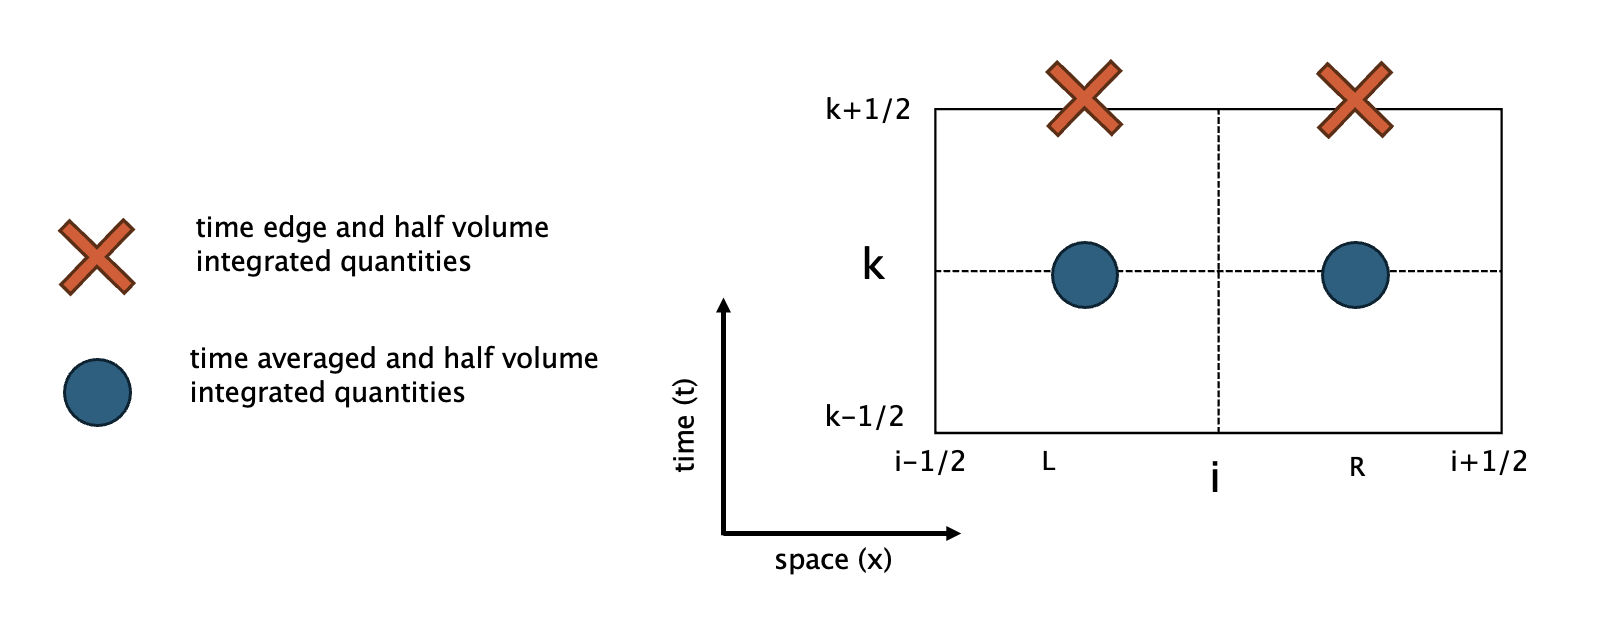
\includegraphics[width=\textwidth]{figures/stencil.png}
    \caption{The discretization stencil}
    \label{fig:stencil}
\end{figure}

%Figure \ref{fig:stencil} shows the stencil location for angular flux and source terms. 

In the traditional source iteration, the scattering source is presumed known from a previous iteration, which leads to the following set of equations to be solved in transport ``sweeps''.
This means that new estimates of both the end of time-step value of angular flux and time-averaged angular flux are computed together in each cell ordinate and group. 
So a $4\times4$ sized system (from stencil values) of equations must be solved to go from cell to cell in each angle.
This process is annoyingly serial over space, but embarrassingly parallel over angles.
The whole system sparse matrix is block (in each ordinate) lower triangular (over all cells).
Source iterations couple angles together in the iterative method by use of the scalar flux.

In OCI, the scattering source is subtracted to the left-hand side, and the information that comes from cells other than cell $j$ is assumed to be known from a previous iteration.
This means that all $4NG$ angular fluxes ($N$ angles, $G$ groups, and stencil values $L$, $R$, $k$, $k+1/2$) are computed simultaneously in cell $j$.
For simple corner balance in slab geometry, this means there is a local $4NG \times 4NG$ system of equations to be solved in each cell.


\subsection{Fourier Analysis}

To ensure that our combination of higher-order discretization schemes is still unconditionally stable, we performed a Fourier analysis to find the slowest-converging mode of the method.
Assuming no scattering, no sources, homogeneous, mono-energetic problem, and make physical assumptions (only positive values of $\Delta x$, $\Delta t$, $\Sigma$, and $v$) we derived the space-time discritization scheme's eigen-function and numerically solve it (see Appendix~\ref{app:therefore}).
% \begin{subequations}
% \begin{align}
%     \psi_{k+1/2,j,L} &= \theta^{k+1}a e^{i\omega j}
%     &
%     \psi_{k+1/2,j,R} &= \theta^{k+1}b e^{i\omega j}
% \end{align}
% \begin{align}
%     \psi_{k,j,L} &= \theta^{k}c e^{i\omega j}
%     &
%     \psi_{k,j,R} &= \theta^{k}d e^{i\omega j}
% \end{align}
% \begin{align}
%     \psi_{k-1/2,j,L} &= \theta^{k}a e^{i\omega j}
%     &
%     \psi_{k-1/2,j,R} &= \theta^{k}b e^{i\omega j}
% \end{align}
% \end{subequations}
% where $k$ is the mode number, $i$ is the imaginary number, $\omega$ is the frequency of the mode, $\theta$ is the , and $j$ is the specific cell.
% Substituting our ansätze into Eqs.~\eqref{eq:scb-mb-a}, \eqref{eq:scb-mb-b}, \eqref{eq:scb-mb-c}, and \eqref{eq:scb-mb-d}, respectively, we
% When this system is solved for its eigenvalues ($\Lambda$) numerically it shows that a MB-SCB scheme is unconditionally stable over $\mu \in [-1, 1]$.  

\subsection{Verification using method of manufactured solution}

Finding benchmark problems that simulate transient, energy dependent, single dimension solutions to the neutron transport equation is difficult \cite{roy_review_2005}.
I used the method of manufactured solutions (MMS) to derive my own benchmark \cite{nse_mms_warsaw}.
It is widely accepted in the field and has previously been used to verify other deterministic neutron transport codes including the production code solver MOOSE \citep{wang_application_2018,moosemms}.

MMS follows a backward solving technique where a solution is made-up---expressing any desired behavior (e.g., smoothness, differentiability, positivity)---then inserted into the governing equation and solved for the source term.
The manufactured source is supplied to the solver to verify that it converges to the correct solution. %at the expected rate. 
To implement MMS I start with a manufactured continuous functional representation of the angular flux in angle, space and time adapted from Eq.~(7) in reference \cite{wang_application_2018} for time dependence.
When moving to multi-group two equations will be used to define the flux in group one and two with the group to group scattering operator linking them together.
%\begin{subequations}
%    \label{eq:manufactured_sol}  
%    \begin{align}
%        \psi_1(x,t,\mu) = (1-\mu^2)\sin(\pi x)e^{-t} \label{eq:af_mms_cont1}\\
%        \psi_2(x,t,\mu) = (1-\mu^2)(-x^4 + x + 1)e^{-t/2} \label{eq:af_mms_cont2}
%    \end{align}
%\end{subequations} 

These equations can now be inserted into the NTE (Eq.~\eqref{eq:sn_nte}) and solved for a continuous functional representation of the source $Q$.
From there the source equations are placed on the stencil by averaging (via numerical integration) in space and time where necessary (see figure \ref{fig:stencil}).
This discretized set of sources is then supplied to the solver and the converged angular flux it provides is then compared to the original manufactured source (again placed on the stencil).
%The range we will be solving these equations is $x \in [0,1]$, $t \in [0,5]$ and $\mu \in [-1,1]$.
%Now we take \ref{eq:af_mms_cont1} and \ref{eq:af_mms_cont2} and insert them into the $S_N$ slab wall neutron transport equation defined in Eqn. \ref{eq:sn_nte} 
%\begin{subequations}
%        \begin{multline}
%            \frac{1}{v_1} \frac{\partial \psi_1(x,t,\mu)}{\partial t} + \mu \frac{\partial \psi_1 (x,t,\mu)}{\partial x} + \Sigma_1\psi_1(x,t,\mu)\\ 
%            =\frac{1}{2} \left(  \Sigma_{s,1} \int^1_{-1}\psi_1(x,t,\mu) \partial \mu + \Sigma_{s,2\rightarrow 1} \int^1_{-1}\psi_2(x,t,\mu) \partial \mu + Q_1\right) 
%        \end{multline}
%        and
%        \begin{multline}
%            \frac{1}{v_2} \frac{\partial \psi_2(x,t,\mu)}{\partial t} + \mu \frac{\partial \psi_2 (x,t,\mu)}{\partial x} + \Sigma_2\psi_2(x,t,\mu)\\ 
%            =\frac{1}{2} \left(  \Sigma_{s,2} \int^1_{-1}\psi_2(x,t,\mu) \partial \mu + \Sigma_{s,1\rightarrow 2} \int^1_{-1}\psi_1(x,t,\mu) \partial \mu + Q_2\right) 
%        \end{multline}
%\end{subequations}
%which yields continuous functional representations for solutions a source term,
%\begin{subequations}
%        \begin{equation}
%            Q_1(x,t,\mu) = \frac{2}{v_1} + 2\mu + 2\Sigma_1(\mu + t + x) - \Sigma_{S,1}(2t + 2x) - 2\Sigma_{S,2\rightarrow1}tx^2 
%        \end{equation}
%        and
%        \begin{equation}
%            Q_2(x,t,\mu) = \frac{2x^2}{v_2} + 4\mu tx + 2\Sigma_2(\mu + tx^2) + \Sigma_{S,1\rightarrow2}(2t + 2x) - 2\sigma_{S,2}tx^2
%        \end{equation}
%\end{subequations}
%Note that these equations are fully defined by independent variables and material data.


\subsection{Implementation in code}

I use the ROCm compute library to solve the system of equations.
Modern GPU vendor-supplied LAPACK libraries often include a \texttt{strided\_batched} class of solvers.
These will operate on a group of like-sized systems in unison and are optimized by the vendors of the hardware themselves.
For example, LU decomposition with pivoting (the most generic direct solver for a system of linear equations) is implemented using rocSOLVER \texttt{strided\_batched\_dgsev} \cite{rocsolver}.
Direct solvers are used in this work.
Currently all systems are assumed dense which for OCI might not be prudent.
Future work could look into using sparse direct solvers which are similarly available as their dense siblings.
%Spare direct solvers could be utilized in the future to decrease memory footprint of OCI schemes specifically.
This makes the use of a strided batched implementation of LU decomposition with pivoting ideal.
Furthermore in this work once that system is solved the return of the A matrix is automatically the decomposition: $L+U+D$.
In subsequent iterations this system can be back solved very quickly again using library functionality (RQ1).
For both schemes the entire convergence loop was executed on the GPU (see appendix \ref{app:therefore}).
Profiling was used to ensure that both sets of compute kernels where performant.

\subsection{Exploration of acceleration scheme}
\label{ssec:method_acc}

This section discusses ongoing work: the derivation of an acceleration scheme for OCI in the thin limit.
When working with iterative schemes, it becomes useful to define systems in operator notation.
The NTE can be written generally as
\begin{equation}
    H\psi = q
\end{equation}
where $H$ is the transport operator, $\psi$ is the unknown function for angular flux and $q$ is some source.
To solve this equation H can be split into components that make sense given the NTE, then lagging and leading components can be established (assuming a fixed point iteration).
How the operator is split is what differentiates OCI from SI.
For example if $H = L-S$ where $L$ is the left hand side of the transport equation and $S$ is the scattering operator and lag the angular fluxes on the scattering operator,
\begin{equation}
    L\psi^{l+1} = S\psi^l + q
\end{equation}
which is a source iteration where $L$ = streaming thru space and time and total absorption operator, %\\ ($\mu_m\frac{\partial\psi}{\partial x} + \frac{1}{v}\frac{\partial\psi}{\partial t} + \Sigma \psi$)
$S$ is the scattering operator (discrete-to-moment operator) which couples all the simultaneous PDEs in angle and group together, %\\($\Sigma_s \int^1_{-1}\psi\partial\mu = \Sigma_s \sum_{n=0}^{M}w_n\psi_n = \Sigma_s\phi$)
$\psi$ angular flux (dependent variable of interest), and
$q$ is the fixed material source.
This is where Rosa, Warsaw, and Perks (2013)~\cite{rosa_cellwise_2013} start in there anylisys of OCI which they call cellwise-bJ.
OCI works by lagging the incident cell wall fluxes of the neighboring cells.
Those fluxes come from the upstream closure that transport solvers use.
Thus it is convenient to further split L,
\begin{equation}
    L = L_c + L_b
\end{equation}
where $L_c$ are the angular fluxes within a mesh cell and $L_b$ are the angular fluxes incident to the mesh cell's surface (boundary).
    %\\($\mu_m\psi_b\frac{dA}{dx} + \frac{1}{v}\psi_b\frac{dA}{dx}$)
Note that what $L_b$ actually consists of depends on the spatial discretization.
After this operator splitting Eq.~\eqref{eq:operator_nte} now becomes
\begin{equation}
    \psi[I+(L_c-S)^{-1}L_b] = (L_c-S)^{-1}q
\end{equation}
where $I$ is the identity matrix.
When OCI's prescribe of what lags (incident fluxes on the surface of the cell) is used this becomes
\begin{equation}
    \label{eq:itter}
    \psi^{(l+1)} = (L_c-S)^{-1}(-L_b\psi^l+q)
\end{equation}

When looking for an acceleration scheme examining the structure of $L_b$ becomes important.
In my research I use the TDMB+SCB discretization for time dependent single dimension multi-group Sn problems (see Eq.~\eqref{eq:tdmb+scb}).
If the angular fluxes from the boundary of the cell are identified (denoted by $j\pm1/2$) $L_b$'s structure can be generally identified.
It should be something like $\pm\mu_m$ filled along four diagonals with every 4$^{th}$ space filled.
This is also vaguely similar to how the SI equations look if formed as a lower triangular system.
In higher dimensions I expect the structure to remain mostly the same for rectilinear grids but might get more complex for unstructured meshes where surface areas may become an issue.

Next I examine the within cell operator: $L_c$.
$L_c$ contains the differential and absorption terms from the NTE.
Also, OCI's converge rate decays in the thin limit due to a-synchronicity \cite{rosa_cellwise_2013, hoagland_hybrid_2021}, which is indicated by a small mean-free path (MFP).
So a small MFP leads to a large condition number of our iteration matrix, thus slow convergence.
To isolate this term I use operator splitting again
\begin{equation}
    L_c = K_d + K_a
\end{equation}
where $K_d$ is the differential operators and
\begin{equation}
    K_a = \frac{\Delta x \Sigma}{2}  I
\end{equation}
is the absorption term.
$K_a$'s structure is simple and clear from the equations \ref{eq:tdmb+scb}.
I could pull out a solitary $\Sigma$ but in this form I can identify that
\begin{equation}
    K_a = \frac{\text{MFP}}{2}  I
\end{equation}
Pushing forward I break up our equations into a standard synthetic approach.
I start with Eq.~\eqref{eq:itter} but recast it with some of the expansions identified,
\begin{equation}
    \psi^{l+1}(K_d + \delta I - S) = (-L_b\psi^l + q)
\end{equation}
where $\delta=$ MFP$/2$.
Now the associated equation for the iteration error is,
\begin{equation}
    (K_d + \delta I-S) f^{l+1} = -L_b f^l
\end{equation}
where $f^{l+1} = \psi^{\text{converged}}-\psi^{l+1/2}$ and $f^{l} = \psi^{\text{converged}}-\psi^{l}$.
Note that this equation is exact in it's current forum.
Now $-L_bf^{l-1}$ is subtracted from both sides:
\begin{equation}
    (K_d + \delta I - S + L_b)f^{l+1} = L_b(f^{l+1}-f^l)
\end{equation}
Notably if everything re-combined Eq.~\eqref{eq:itter} is reformed.
So a synthetic acceleration system starting with Eq.~\eqref{eq:itter} rewritten for half steps is
\begin{subequations}
    \begin{equation}
        \label{eq:acc1}
        \psi^{(l+1/2)} = (L_c-S)^{-1}(-L_b\psi^l+q)
    \end{equation}  
    the associated equation for mid step error
    \begin{equation}  
        \label{eq:acc2}
        f^{l+1/2} = -M L_b(\psi^{l+1/2}-\psi^l)
    \end{equation}  
    and the definition of the errors
    \begin{equation}  
        \label{eq:acc3}
        \psi^{l+1} = \psi^{l+1/2} + f^{l+1/2}
    \end{equation}
\end{subequations}
where,
\begin{equation}
    M \approx (K_d + \delta I + L_b - S)^{-1}
\end{equation}
and is easier to obtain then the actual inverse.
Note that equation 3 from ref \cite{tsa2009rosa} is the recombined version of Eq.~\eqref{eq:acc2}.
From here estimations can be made about what a good approximate of $M$ will be in the conditions where Eq.~\eqref{eq:acc1} degrades.
%If we actually inverted $H$ this would just be another transport step.
%Note that we can relate this idea of synthetic acceleration to preconditioning by noting
%\begin{equation}
%    P \equiv I + M(I-H)
%\end{equation}
%From here I take some stabs at identifying what reasonable values for $M$ could be.
%When we ask our selves "what should M be" we could just as easily pose the more pessimistic analog: "why or, where rather, does H suck to invert".
%This is where our knowledge about the thin limit comes in.
%We know H is painful to invert when $\delta I$ is small as that is a problem in the thin limit where cell wise communication becomes dominant.
%When $\delta I$ is small a good conservative approximation for M may become
%\begin{equation}
%    H^{-1} \approx M = (K_d + L_b - S)^{-1}
%\end{equation}
%but we just converged our within-cell scattering, time rate of change, and steaming operators from the transport step so lets assume we have a good estimate of that.
%We can also assume that the boundary information coming into every cell will blah likewise lets scoot that and all we are left with is the differential operators (from a discretization scheme)
%\begin{equation}
%    H^{-1} \approx M = (K_d)^{-1}
%\end{equation}
%which makes the full mid step solution
%\begin{equation}
%    \label{eq:m}
%    -K_d^{-1}*L_b
%\end{equation}
%This leads to the suggestion at the possible algorithm
%\begin{enumerate}
%    \item transport step as described in eq. \ref{eq:acc1}
%    \item mid step corrector (eq. \ref{eq:acc2}) with . This will look like a transport in every angle
%    \item colsure from eq
%\end{enumerate}
%But Joanna, your probably asking yourself. 
%This just using a cheap sweep between every OCI transport iteration
%I say in 1D
%in higher dimensions this will look like a \textit{a ray trace} something GPUs are literally built for.

%From here more work is need to be down to conduct Fourier analysis in both with and with out the discretization scheme

%What ever scheme is used it can be supplemented by GMRES

\section{Monte Carlo transport methods}
As in the previous section the methods employed are further described in attached publications in the appendix.
They are briefly summarized here.

%   
\subsection{Python-based portability for rapid methods development}

A software engineering scheme was developed and deployed in Monte Carlo/Dynamic Code \cite{morgan_monte_2024} using the Numba compiler for Python \cite{lam_numba_2015}, mpi4py \cite{mpi4py_2021}, and an a-synchronous GPU event scheduler called Harmonize \cite{brax2023} (See Appendix~\ref{app:cise}).
MC/DC can run the same set of physics functions written by subject-area experts in the Python interpreter or compiled to x86-64, ARM64, and Power9 CPUs as well as AMD and Nvidia GPUs.
All compilation targets also support the use of MPI to distribute work to multiple nodes of an HPC.
It is a demonstration of portability using a high-level language coupled to a portability framework to enable rapid methods development.

\subsection{Delta tracking in MCATK and MC/DC}

In MCATK a hybrid delta-surface tracking scheme was developed and deployed (See Appendix~\ref{app:hybridmcatk}).
I initially implemented this scheme (my work is fully described by the publication included in Appendix \ref{app:hybridmcatk}), but it has been extended by others and is shipped in current production versions of MCATK.
The point of the delta-surface tracking scheme in MCATK is entirely to avoid extra expensive macroscopic cross section lookups.
It still conducts surface tracking on mesh.
After implementation the hybrid delta-tracking scheme was tested in both k-eigenvalue and fixed source transient simulations using the
\begin{itemize}
    \item HEU-MET-FAST-086 benchmark of Godiva IV \cite{godivaiv2021}, and
    \item Measurement of Uranium Subcritical and Critical IER 488 (MUSiC) experiment \cite{music2021}.
\end{itemize}
Runtime and errors were then compared to draw conclusions.
This work was published in a conference publication \cite{morgan2023oci} (see Appendix~\ref{app:hybridmcatk}).

In MC/DC I propose a slight alteration to the hybrid-scheme developed and deployed in my previous work in MCATK.
Current versions of MC/DC do not stop particles at mesh crossings when using surface tracking and use a track-length estimator to tally impacts to multiple cells at once.
Using this tally algorithm already in MC/DC, delta tracking could be used in conjunction with the track length estimator as in the previous work in MCATK.
However the proposed algorithm in MC/DC will more closely resemble the vanilla delta tracking algorithm and not stop particles at now cell \textit{and} surface crossings.
Other quantities of interest will be tallied with collision estimator as the specific material data is required for values like fission reaction rate.
This will require additional computational burden but the hope is that the new tally functionality in MC/DC is sufficiently optimized to still allow this scheme to be more performant.

To evaluate the delta tracking scheme as compared to surface tracking I will use figure of merit (FOM) values.
FOMs are constructed to observe impact of a variance reduction technique on both variance (as computed by the Monte Carlo scheme) and on runtime (as many variance reduction schemes incur additional computation burden).
The most common figure of merit and the one I will employ is simply
\begin{equation}
    FOM = \frac{1}{\sigma^2 t_{wc}}
\end{equation}
where $\sigma^2$ is the variance as already computed by MC solvers and $t_{wc}$ is the total wall-clock-runtime.
Using this metric (higher is better) variance reduction shames can be compared to each other and the analog solver.
I propose using this metric to evaluate the impact of the hybrid-delta tracking scheme 
I plan to initially verify the tracking algorithm in MC/DC using the AZURV1 benchmark problem \cite{ganapol_homogeneous_2001}.
Then compare figures of merrit on problems of interest.
Potential problems of interest include:
\begin{enumerate}
    \item Dragon burst problem \cite{kimpland2021dragon};
    \item C5G7 Small modular reactor \cite{jia_hou_oecdnea_2017}; and
    \item Kobyashi void dog-leg void problem (multigroup and contentious energy simulations) \cite{Kobayashi2001}.
\end{enumerate}
\chapter{Preliminary Results}
\label{ch:results}

\section{Deterministic transport}

\subsection{Verification and analysis of discretization scheme}

I found that the MB-SCB scheme is unconditionally stable over $\mu \in [-1, 1]$. While experimenting with this method we did find that, under some conditions, it can produce negative fluxes; however, the negative flux oscillations were critically damped and dissipated with time.

I initially implemented MMS in a mono-energetic problem slab wall problem with $L=1$cm, $\Sigma$=0.5/cm, $t_0=0$s, $\Delta t = 0.1$s, $\Delta x=0.01$cm, $v=5$cm/s, $\Sigma_s=0.1$/cm, $\psi_0=\psi_m(t=0,x,\mu)$, $\psi_{x=0}=\psi_m(t,x=0,\mu)$, $\psi_{x=L}=\psi_m(t,x=L,\mu)$, in S$_{32}$.
All presented numerical investigation used a convergence tolerance of \num{1e-9} and controlled for false convergence using an on the fly estimate of spectral radius.
Figure \ref{fig:mms_sol} shows the manufactured and solver solutions matching through time.
Work is ongoing to extend this to a multi-group simulation and to use the manufacture solution to show convergence rate.


\begin{figure}[h!]
    \centering
    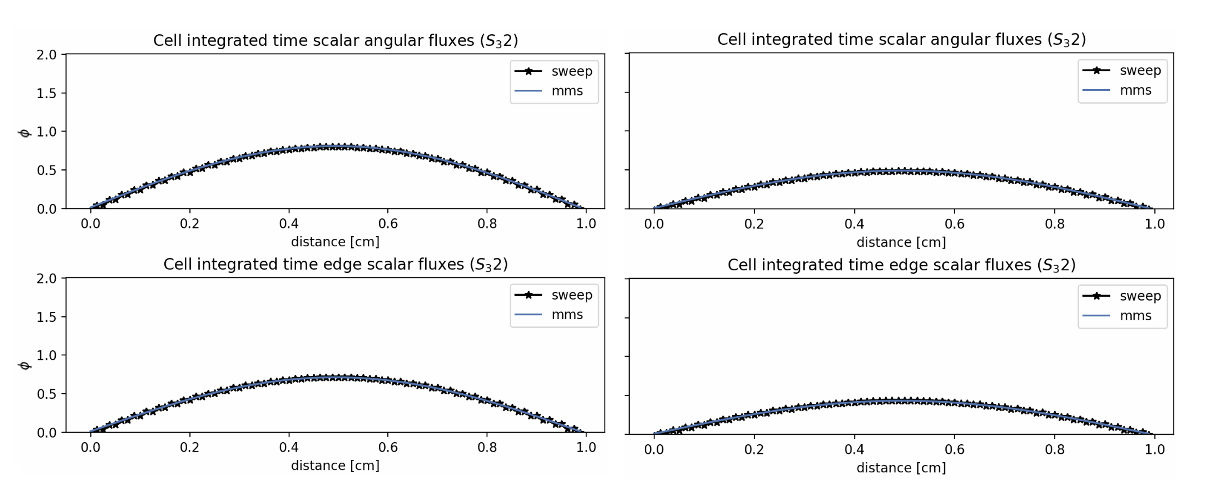
\includegraphics[width=.75\textwidth]{figures/results/mms_sol.png}
    \caption{The manufactured and solver solutions thru time.}
    \label{fig:mms_sol}
\end{figure}

%A bug exists somewhere in the current code that prevents the use of the MMS solution to also confirm order of convergence of the discritization scheme.
To verify the order of convergence of the spatial discritization an over resolved solution (at $\Delta x=\num{1e-4}$) from the solver is generated.
Error is compared at the midpoint which discritization chosen such that the midpoint is always in the same location.
Figure \ref{fig:conv_rate} shows the convergence over various choices of $\Delta x$ and shows that the scheme is second order.
Work is ongoing to confirm the order of time discritization scheme using this method.

\begin{figure}[h!]
    \centering
    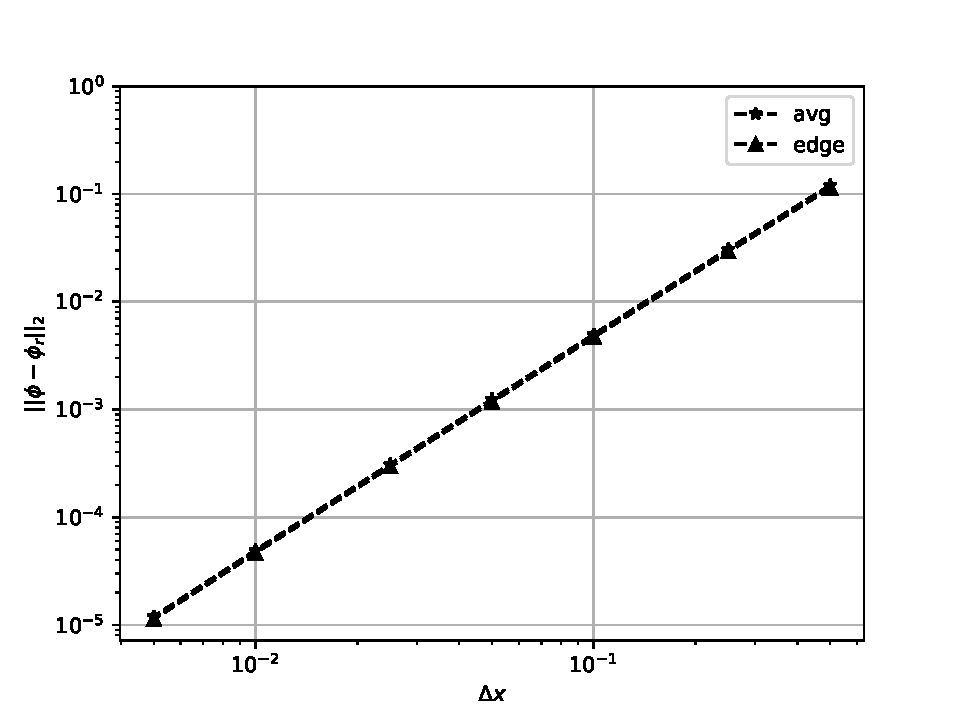
\includegraphics[width=.5\textwidth]{figures/results/convergance_rate.pdf}
    \caption{Spatial convergence rate of the discritization scheme using an over resolved $\phi_r$ solution to scalar flux from the solver.}
    \label{fig:conv_rate}
\end{figure}


\subsection{Performance Results}

Rosa, Warsa, and Perks~\cite{rosa_cellwise_2013} describe a test problem they used to validate Fourier analysis of their 2D steady state solver.
I adapt it to the 1D time dependent regime and use it to conduct preliminary performance evaluations.
Figure \ref{fig:rosa_test} shows a simple slab wall problem with vacuum boundary conditions and table \ref{table:rosa_test} lists the material data and solver parameters.
The initial condition is $\psi_{t=0} = 0$, and the time step $\Delta t = 0.1$ s.
Future work might explore more complex problems either with more groups or with material heterogeneity.

\begin{figure}[h!]
    \centering
    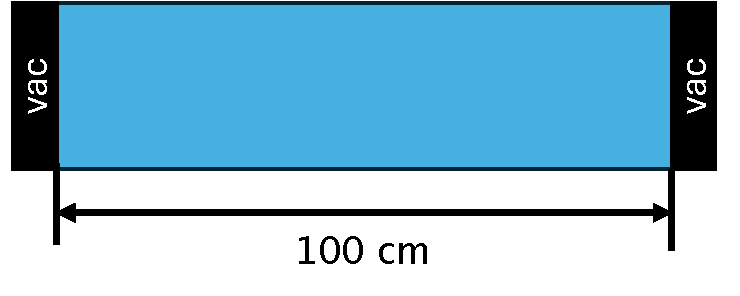
\includegraphics[width=.4\textwidth]{figures/results/rtest.pdf}
    \caption{Rosa test problem}
    \label{fig:rosa_test}
\end{figure}

\begin{table}[!htb]
  \centering
  \caption{Rosa test problem material data and simulation parameters.}
  \begin{tabular}{c c c c c c  } \hline 
    Property & Group 1 & Group 2 & units \\ \hline
    $\Sigma$ & 1.5454 &  0.45468 & cm$^{-1}$  \\
    $\Sigma_{s,g\rightarrow g}$  & 0.61789 &  0.0072534 & cm$^{-1}$  \\
    $\Sigma_{s,g'\rightarrow g}$  & 0.38211 &  0.92747 & cm$^{-1}$ \\
    $Q$ & 1 & 1 & cm$^{-3}$s$^{-1}$\\
    $v$ & 1 & 0.5 & cm s$^{-1}$ \\
    \hline
  \end{tabular}
  \label{table:rosa_test} 
\end{table}


Figure~\ref{fig:perf} at left compares the wall clock runtime of OCI (in black) and SI (in blue) over various selections of MFP (controlled via $\Delta x$ spatial discretization) and quadrature orders.
The total time to convergence was collected on the third time step to allow the GPUs to "spin up" with the initial iteration guess being 0 at every time step.
In normal compute mode this would be done with the solution from the previous time step.
Again note that the runtimes presented here are the on-GPU time in the convergence loops (see appendix \ref{app:therefore}).
The total cross section used in the MFP scale is the limiting value (the smallest) from group 2 (see Table~\ref{table:rosa_test}).
SI increases linearly as the cells get optically thinner.
The number of iterations required to converge the solution is the same but the size of the solution is getting larger.
SI only has $N_{\text{angle}}$ of $4\times 4$ systems to solve at any given moment so the amount of serial work increases with the number of cells (by decreasing $\Delta x$).
However as we increase quadrature order the runtime performance of SI actually improves as more degrees of freedom are more readily parallelized by the solvers.

\begin{figure}[h!]
    \centering
    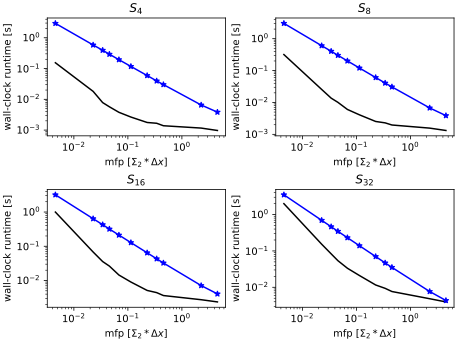
\includegraphics[width=.49\textwidth]{figures/results/runtime.png}
    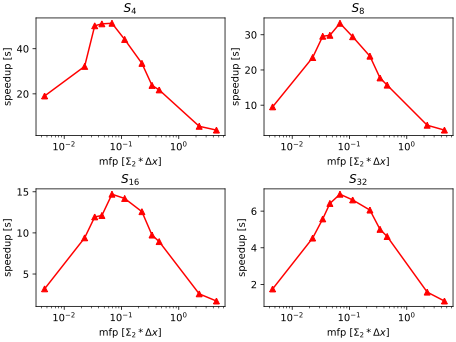
\includegraphics[width=.49\textwidth]{figures/results/speedup.png}
    \caption{Wall clock runtime of OCI black and SI red (left) and speedup (right) of Rosa et al.~\cite{rosa_cellwise_2013} test problem over choice of mean free path in various quadrature orders}
    \label{fig:perf}
\end{figure}

OCI runtime in this problem are more complex.
The degrees of freedom that can be parallelized increases with the number of cells (by decreasing $\Delta x$) however the spectral radius degrades dramatically as cells get thinner.
OCI requires more iterations to converge the solution but those iterations can be done faster on the GPU.
For OCI there seems to exist an inflection point where the method goes from increasing sub-linearly to super-linearly.
For this problem it seems to fall around mfp$=0.1$ where there are enough cells to saturate the GPU before the thin limit.

Figure \ref{fig:perf} at right shows the speedup of OCI over SI for that same problem. 
The previously mentioned optimal spot can now be seen as a definite peak around MFP$=0.1$.
The peak move slightly depending on the number of angles in quadrature.
I believe this is a feature of the \texttt{strided\_batched} solvers which can behave differently based on the dimension of the underlying matrices\cite{rocsolver}.
In smaller quadrature orders the speedup is the greatest with OCI being about 45 times faster then SI.
As more angles are added to quadrature the speed-up of OCI over SI shrinks as SI is better able to parallelize with more degrees of freedom in angle.
This confirms my previous investigations \cite{morgan2023oci} and Rosa et al.~\cite{rosa_cellwise_2013} results, that parallelizing over the largest dimension is advantageous to computation on GPU.
These conclusions provide insight into research questions 1 and 2.
%add further conclusions

\subsection{Time dependent iterative results}

To explore how time discretization impacts the convergence of OCI and SI we again use with the Rosa test problem.
Figure \ref{fig:time_desc} shows the number of iterations required to converge using both iterative schemes varying the time step, at various selections of $\Delta x$.
Again we observe that SI behaves independently of the MFP (and $\Delta x$) so the blue curve is the same on every plot.
SI does see improved convergence rate with respect to smaller time discretizations which we believe is due to improvements from the scattering ratio ($c=\Sigma_s/\Sigma$).
OCI improves with both larger choices of MFP (due to a-syncronisty) and smaller times steps due to both improvments to scattering ratio (as in SI) but now additional do to increased cellular opacity.
In fact the rate of improvement of the convergence rate actually increases in the thin limit.
This confirms our hypotheses from observations of the spectral radius, that for smaller time steps OCI converges more rapidly, especially for problems in the thin limit.
These conclusions go to answer research question 3.
% effectivaly time dependence is an accleration scheme for OCI

\begin{figure}[h!]
    \centering
    \caption{Iteration count of OCI and SI to converge the Rosa problem over various choices of $\Delta t$ and $\Delta x$}
    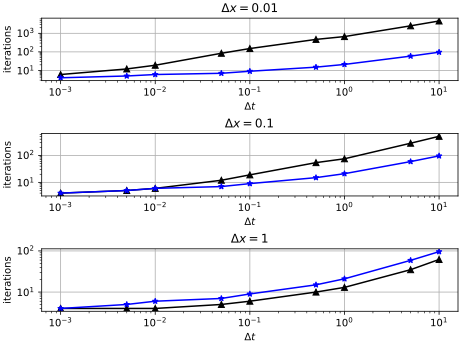
\includegraphics[width=.5\textwidth]{figures/results/time_desc.png}
    \label{fig:time_desc}
\end{figure}

\section{Monte Carlo Methods}

\subsection{MC/DC performance results}

To compare MC/DC to another Monte Carlo neutronics software package, we use a time-dependent version of the Kobayashi dog-leg void-duct problem \cite{Kobayashi2001, variansyah_mc23_mcdc}.
Figure \ref{koby-problem} at left shows the void duct and the location of the neutron source at the opening of the duct.
The initial condition is zero flux everywhere.
Radiation moves down the void quickly and then penetrates into the walls of the problem.
Figure~\ref{koby-problem} at right shows the duct clearly with the scalar flux solution in a time-averaging window of 10 s at somepoint time from MC/DC and OpenMC \cite{romano_openmc_nodate} (an open-source code written in \texttt{C++}) .

\begin{figure*}[h]
    \centering
    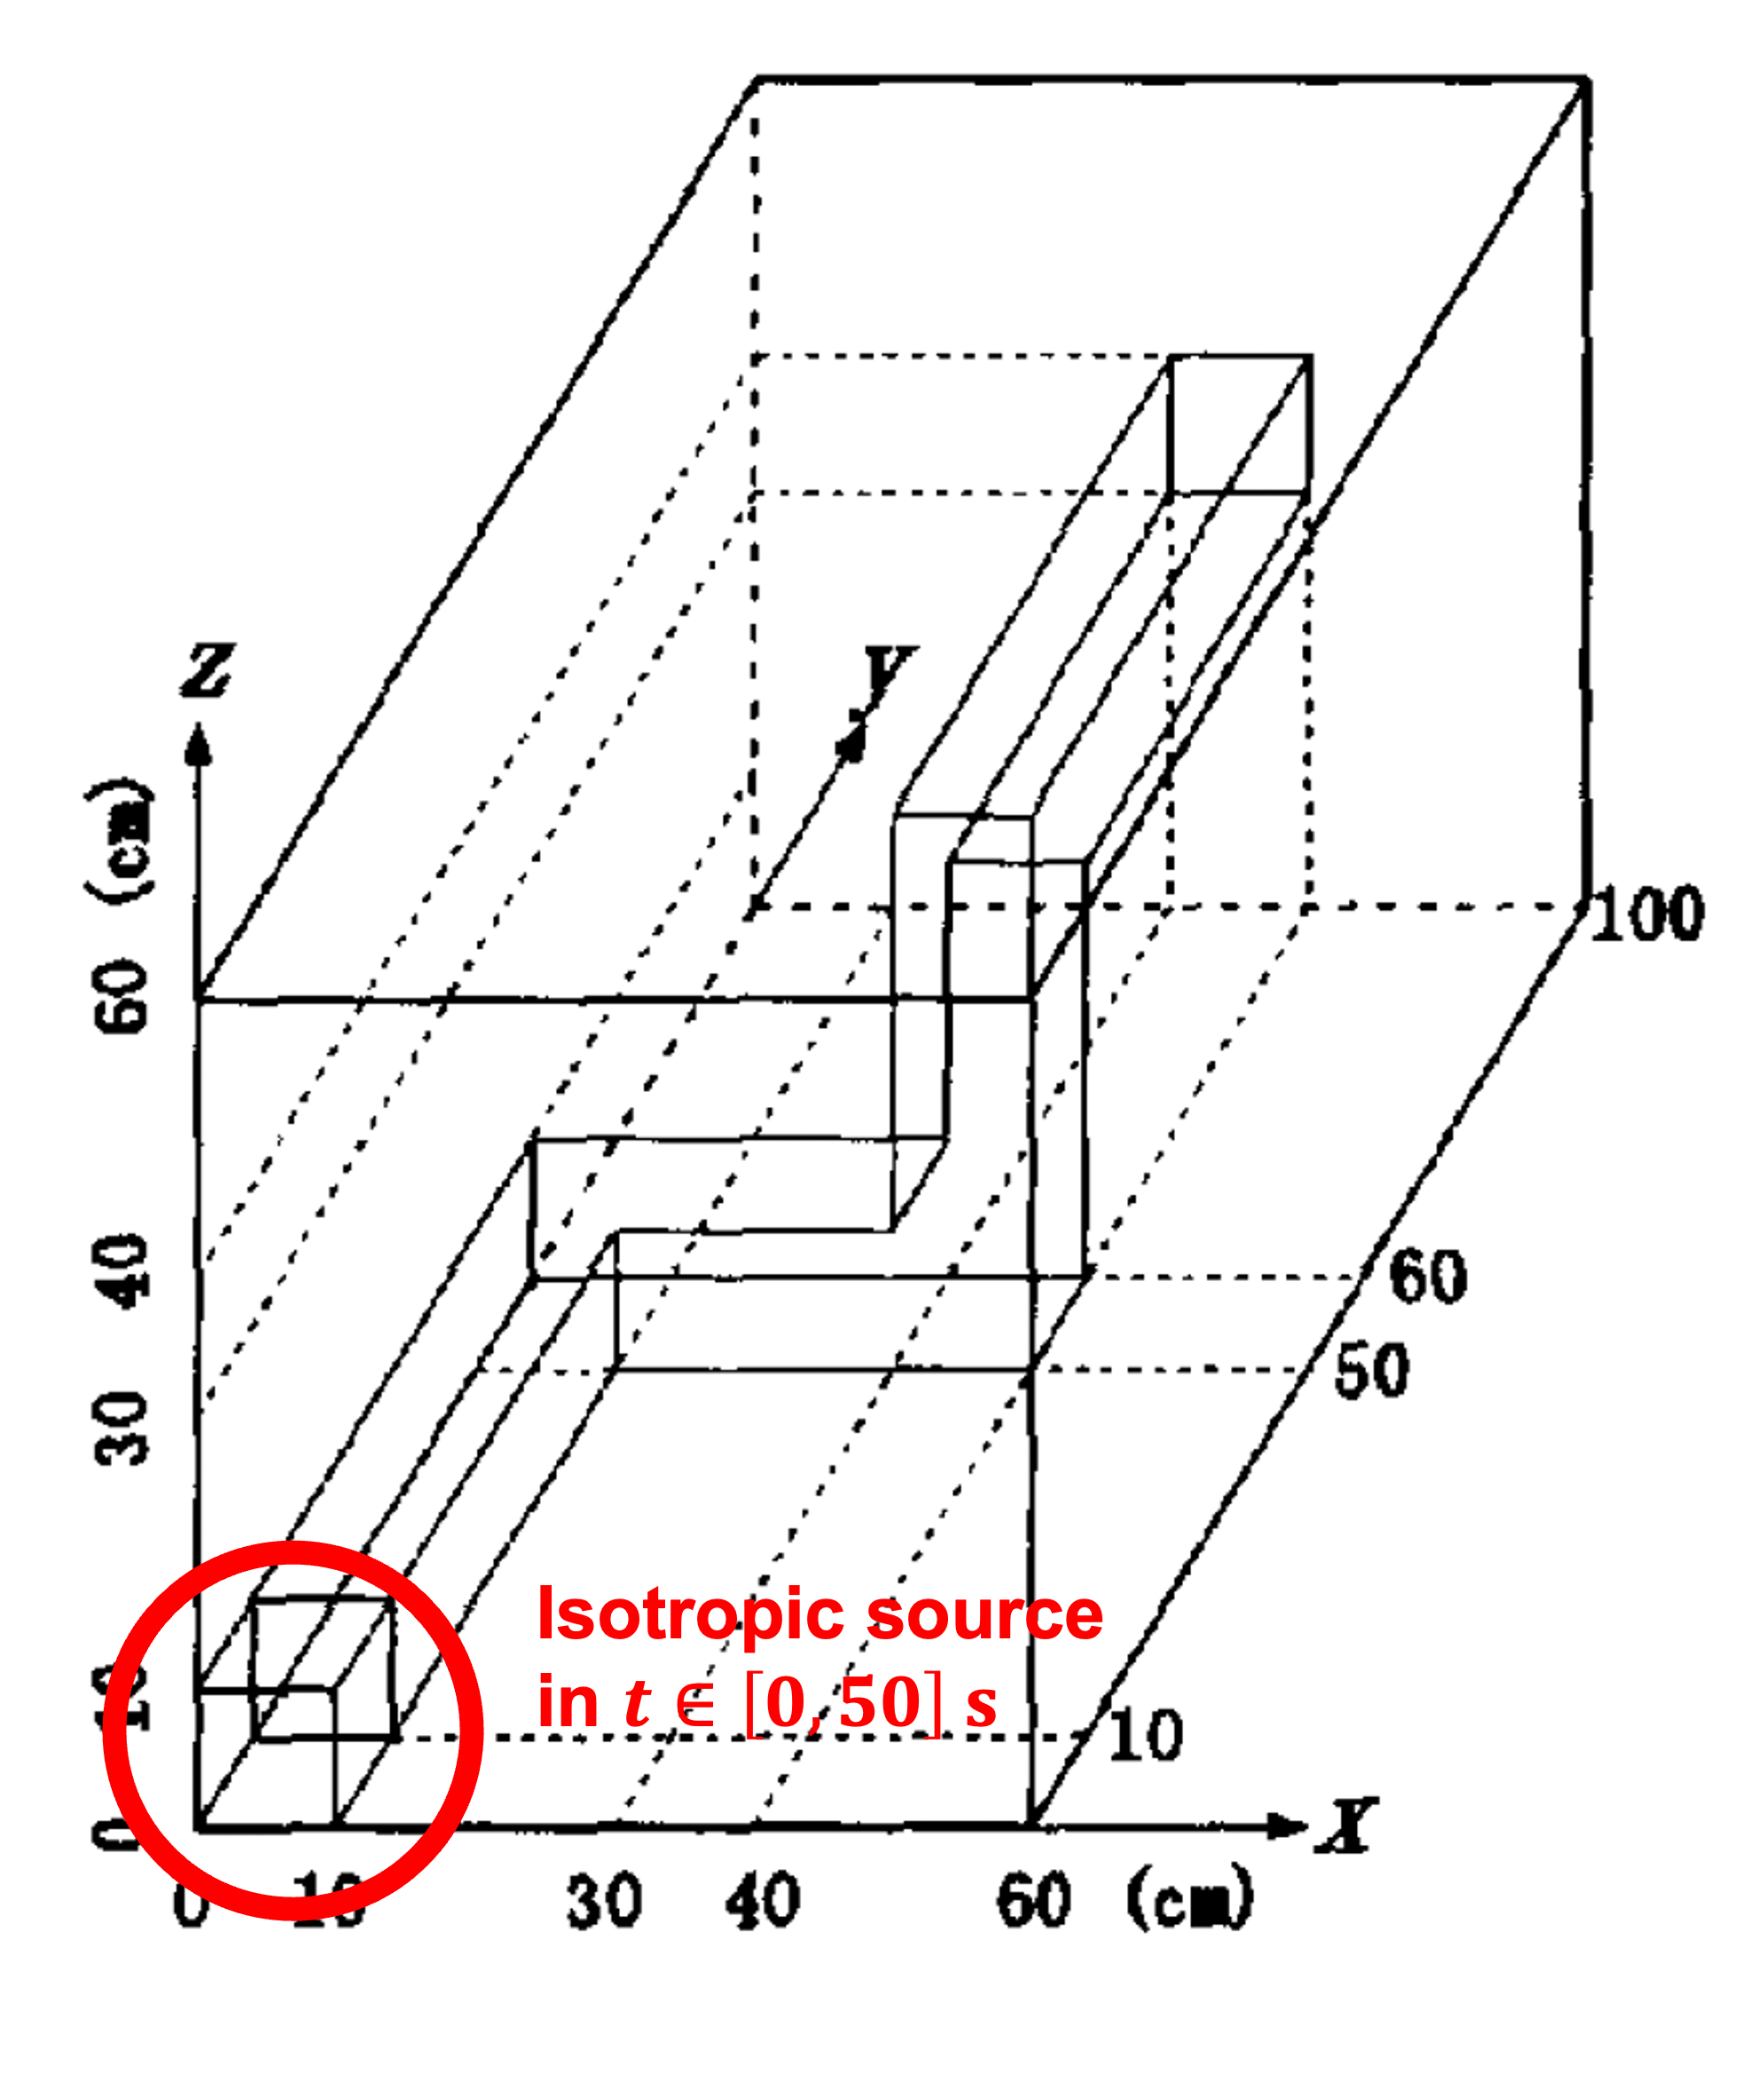
\includegraphics[width=.4\textwidth]{figures/results/kobayashi_problem.png} \hspace{1cm}
    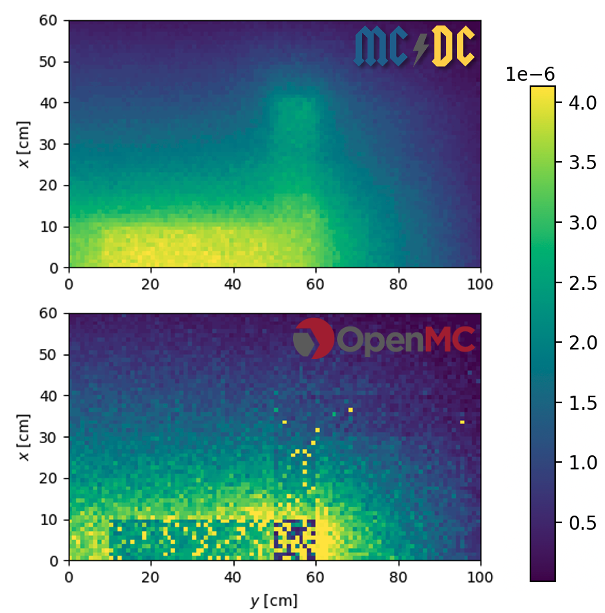
\includegraphics[width=.5\textwidth]{figures/results/koby_mcdcopenmc.png}
    \caption{Left: Kobayashi problem schematic. Right: Time and space averaged scalar flux solution to the Kobayashi problem run with \num{1e9} particle histories from MC/DC (top) and OpenMC (bottom).}
    \label{koby-problem}
\end{figure*}

Figure~\ref{performance_results} at left shows the runtime results of MC/DC compared with OpenMC on a single node of the Quartz supercomputer (two socket 18-core Intel Xeon E5-2695 v4) at Lawrence Livermore National Laboratory (LLNL).
Caching in MC/DC was enabled for these results, meaning there is no JIT compilation overhead.
We examine the impact of a variance reduction technique called implicit capture \cite{lewis_computational_1984}, which is supported in both codes.
OpenMC is about 20 times faster than MC/DC for this problem with implicit capture.
Without implicit capture that performance gap falls to 12 times.
This performance gap is due to OpenMC's tracking algorithm, which does not stop particles at mesh crossing events as MC/DC currently does.
OpenMC is currently limited to the use of the collision estimator to estimate the scalar flux spatial distribution in time-dependent simulation, whereas MC/DC uses the track length estimator \cite{lewis_computational_1984}, which is computationally more expensive but yields better statistics.
This is shown in figure~\ref{koby-problem} at bottom right where OpenMC's result has tally cells with a poorly converged solution (displaying as yellow spots) and MC/DC's (top right) doesn't.
Work is ongoing to implement this particle stop command.
When this is enabled, we suspect the performance gaps for this problem will close substantially between MC/DC and OpenMC.

\begin{figure*}[h]
    \centering
    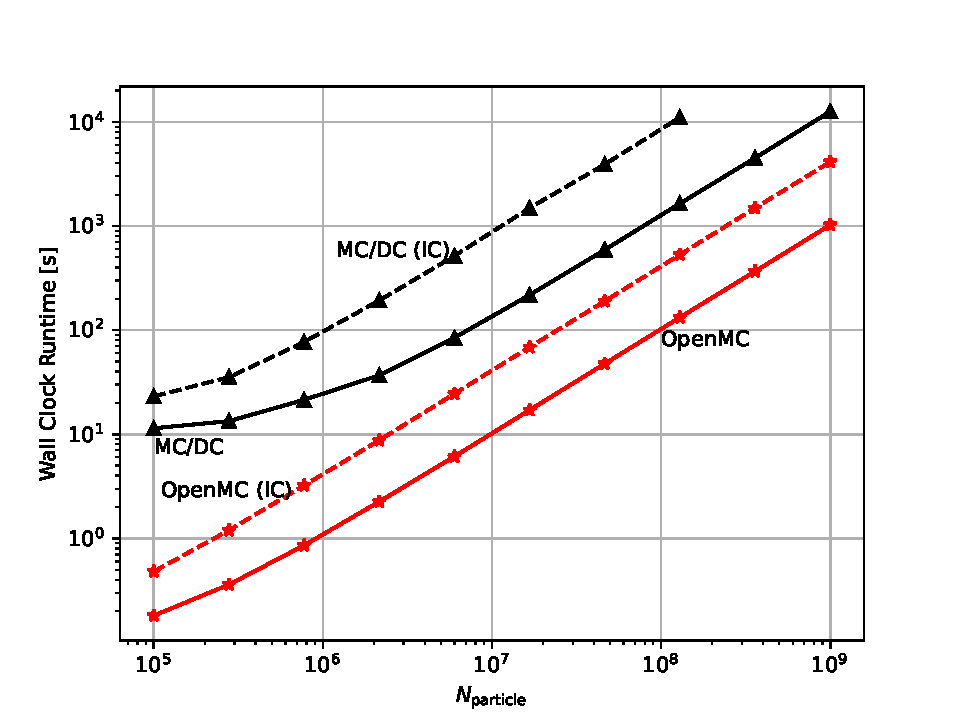
\includegraphics[width=.49\textwidth]{figures/results/code_comparisons.pdf}
    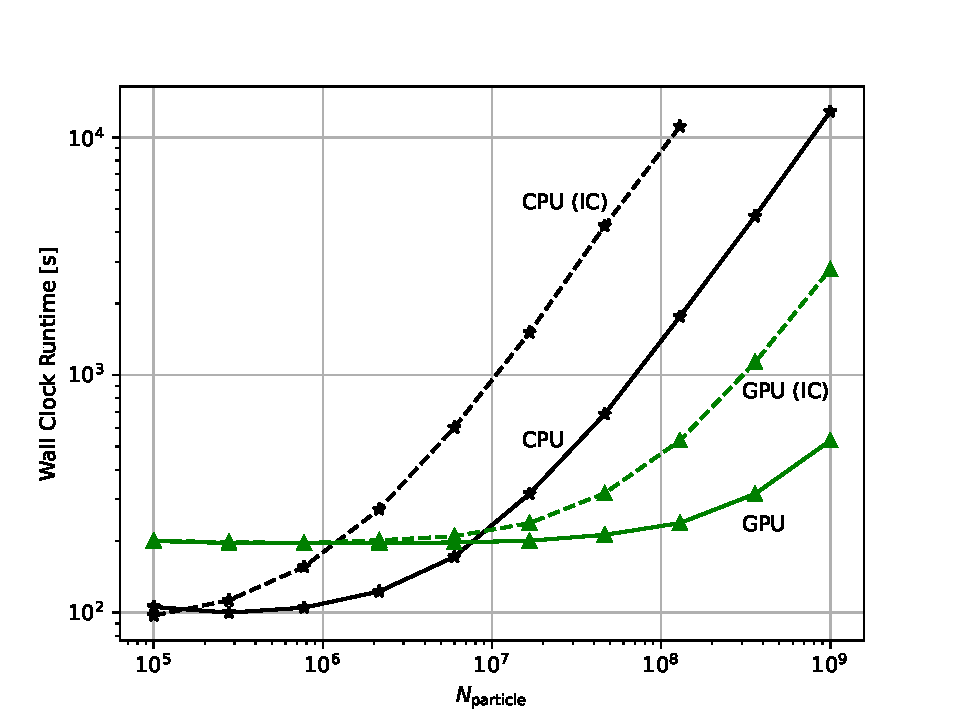
\includegraphics[width=.49\textwidth]{figures/results/mcdc_comparisons.pdf}
    \caption{Left: Wall clock runtime of the Kobyashi problem over particle counts with and without implicit capture (IC) between cached MC/DC (black) and OpenMC (red). 
    Right: Wall clock runtime of the Kobyashi problem over particle counts in uncached MC/DC CPU (black) and GPU (green) modes.}
    \label{performance_results}
\end{figure*}

While these performance results are promising more work is needed to explore MC/DC's (and by extension the software engineering scheme using Numba) performance on modern hardware.
I propose examining the performance of MC/DC more stringently on GPU accelerators including thru the use of code profilers when available.
Also expanding the performance analysis of MC/DC on GPUs to other problems of interest (Dragon burst experiment, C5G7, etc.), other currently enabled GPU types (AMD), and multi-GPU computations.
These initial investigations go to answer research question 1.

\subsection{Hybrid delta tracking in MCATK}

Three experiments where used to confirm that the hybrid delta tracking scheme converged to the expected solution. This was done  via code-to-code comparison
K-eigenvalue simulations were started with 100 inactive cycles before 500 active ones using \num{1e5} particles in each cycle.
Table \ref{table:runtime} shows the performance increase when hybrid-delta tracking is enabled.
The differences in eigenvalue between simulations with and without the hybrid-delta tracking algorithm are all within 1.12 standard deviations. This table also shows a significant speed-up in the over all solve time of MCATK with delta tracking incurring between a 1.54--1.75$\times$ speed-up.

\begin{table}[!htb]
  \centering
  \caption{Benchmark results: where ${\Delta \sigma}$ is the difference in number of standard deviations of ${k_{\text{eff}}}$ between the standard algorithm and hybrid-delta tracking.}
  \label{table:runtime} 
  \begin{tabular}{@{}c c c c c c@{}} \toprule
    Benchmark & MCATK & MCATK & $k$ & $\Delta \sigma$ & speed-up\\
               & Surface (s)  & Hybrid-Delta (s) &  & &\\ \midrule
    \ Godiva Case 5 & 16900 &  10987 & 0.99736 &  -0.747 & 1.54 \\
    \ MUSiC Case 8  & 23937 &  14832 & 0.99970 &  0.130 & 1.61 \\
    \ MUSiC Case 9  & 22649 &  12973 & 0.99929 &  -1.105 & 1.75 \\ 
    \bottomrule
  \end{tabular}
\end{table}


\begin{table}[!htb]
  \centering
  \caption{Benchmark results: where $\Delta \sigma$ is the difference in number of standard deviations of the $\alpha$-eigenvalues between standard algorithm and hybrid-delta tracking.}
  \label{table:runtime_trans} 
  \begin{tabular}{{@{}c c c c c c@{}}} \toprule 
    Benchmark & MCATK            & MCATK         & $\alpha_{\text{avg}}$ & $\Delta \sigma$ & speed-up\\
               & Surface (s)  & Hybrid-Delta (s) & &                 &\\ \midrule
    \ Godiva Case 5 & 2689 &  2168 & \num{-3.54e-3} &  \num{-1.91} & 1.24 \\
    \ MUSiC Case 8  & 4352 &  2665 & \num{-1.26e-3} &  \num{-0.76} & 1.63 \\
    \ MUSiC Case 9  & 4440 &  2786 & \num{-1.02e-3} &  \num{-2.75} & 1.59 \\ 
    \bottomrule
  \end{tabular}
\end{table}

To compute error between tracking schemes in fixed source simulations we used the estimates of the $\alpha$-eigenvalue computed using MCATK's time-dependent algorithm.
The benchmarks were started at \SI{0}{\second} and ran to \SI{500e-8}{\second} with a time step of $\Delta t =$ \SI{1e-8}{\second}.
The particle population was combed between every time step up or down to \num{1e5} particles. 
Table \ref{table:runtime_trans} shows less speed-up then for k-eigenvalue computations (only between 1.24$\times$ and 1.63$\times$) but still significant for minimal alterations to a production code. This table also shows the average $\alpha$-eigenvalues method within three standard deviations.

Hybrid-delta tracking on a structured mesh improves run time in large and materially complex simulations like the ones we benchmarked: 1.5--1.75$\times$ speed-up for k-eigenvalue and 1.2--1.6$\times$ speed-up for fixed source problems.
FOMs where not produced as part of the work in MCATK.
The speedup in MCATK was entirely due to the elimination of extra cross section lookups in an otherwise standard surface tracking algorithm with a track length estimator.
These conclusions go to answer research question 5.

These initial investigations in MCATK gives confidence that when implemented in MC/DC we will also see performance improvements.
When moving towards an implementation in MC/DC we expect a potential speedup (due to eliminated distance to surface computations) but more marginal speedup in materially complex problems.
I do expect that adding  a track length estimator to make the variance very small.
Work in MC/DC is ongoing beginning with the majorant computation functionality.

\chapter{Planned schedule} 
\label{ch-schedule}

My proposed timeline for the remainder of my PhD, included is three additional publications (1) conference proceeding (2025 M\&C) about MC/DC's GPU performance, (2) journal article about deterministic work currently underway, and (3) journal article about investigated acceleration schemes.

\begin{figure}[ht]
    \centering
    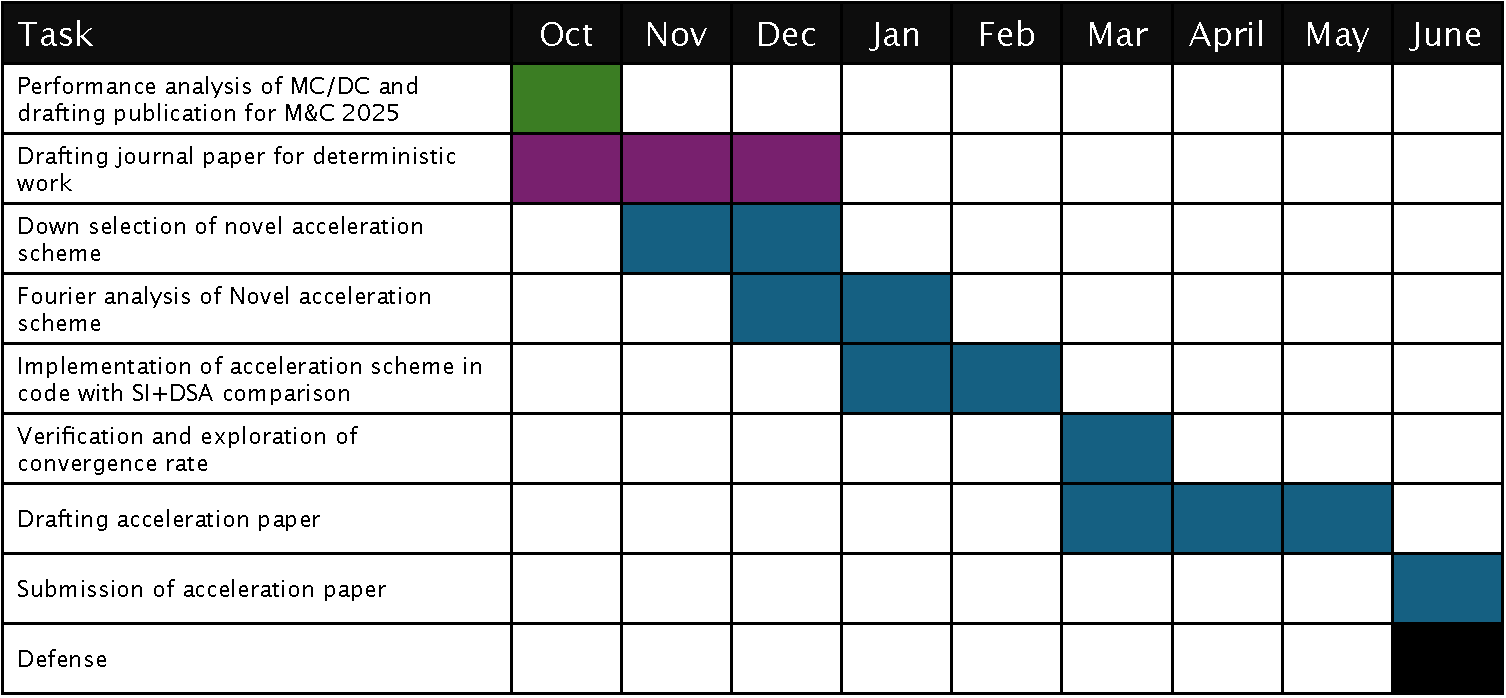
\includegraphics[width=\textwidth]{figures/time_line.pdf}
    \caption{Green and Orange are Monte Carlo work, purple is the first set of deterministic work, blue is the second set of deterministic work focused on finding an acceleration scheme black is defense.}
    \label{fig:gantt}
\end{figure}

 
%----------------------------------------------------------------------------------------
%	APPENDICES
%----------------------------------------------------------------------------------------

\addtocontents{toc}{\vspace{2em}} % Add a gap in the Contents, for aesthetics
\appendix % Starts of appendices

\numberedchapter
\chapter{appendices} \label{appA}

\section{Conference Publication, and Presentation for proposed investigations}


\subsection{OCI Investigations}

Copper Moutian

M\&C 2023

\subsection{Hybrid-Delta Tracking Schemes}

M\&C 2023

\subsection{Acceleration and Abstraction of Python}

SciPy 2024

S3C 2024

Monte Carlo Computational Summit

M\&C 2023

ANS Annual 2022

SciPy 2022

\section{All Publications}

\section{Submitted Draft: Performant and Portable\\ Monte Carlo Neutron Transport via Numba}
\label{app:cise}

This paper was submitted to \textit{IEEE Computing in Science and Engineering} on September 3rd 2024. 
I have not received a response.
A preprint was posted to arxiv and has been the assigned the DOI 10.48550/arXiv.2409.04668.

My coauthors are all members of the Center for Exascale Monte Carlo Neutron Transport (CEMeNT) includes
\begin{itemize}
    \item Ilham Variansyah, PhD (committee member)
    \item Braxton Cuneo, PhD
    \item Todd S. Palmer, PhD (committee member)
    \item Kyle E. Niemeyer, PhD (advisor)
\end{itemize}
As MC/DC is the primary deliverable of CEMeNT it is a deeply combative effort.


%\subsection{My work}
%I was the primary author and as such drafted the whole paper.
%I received significant edits from all my co authors who all contributed to the work.
%I collected the data

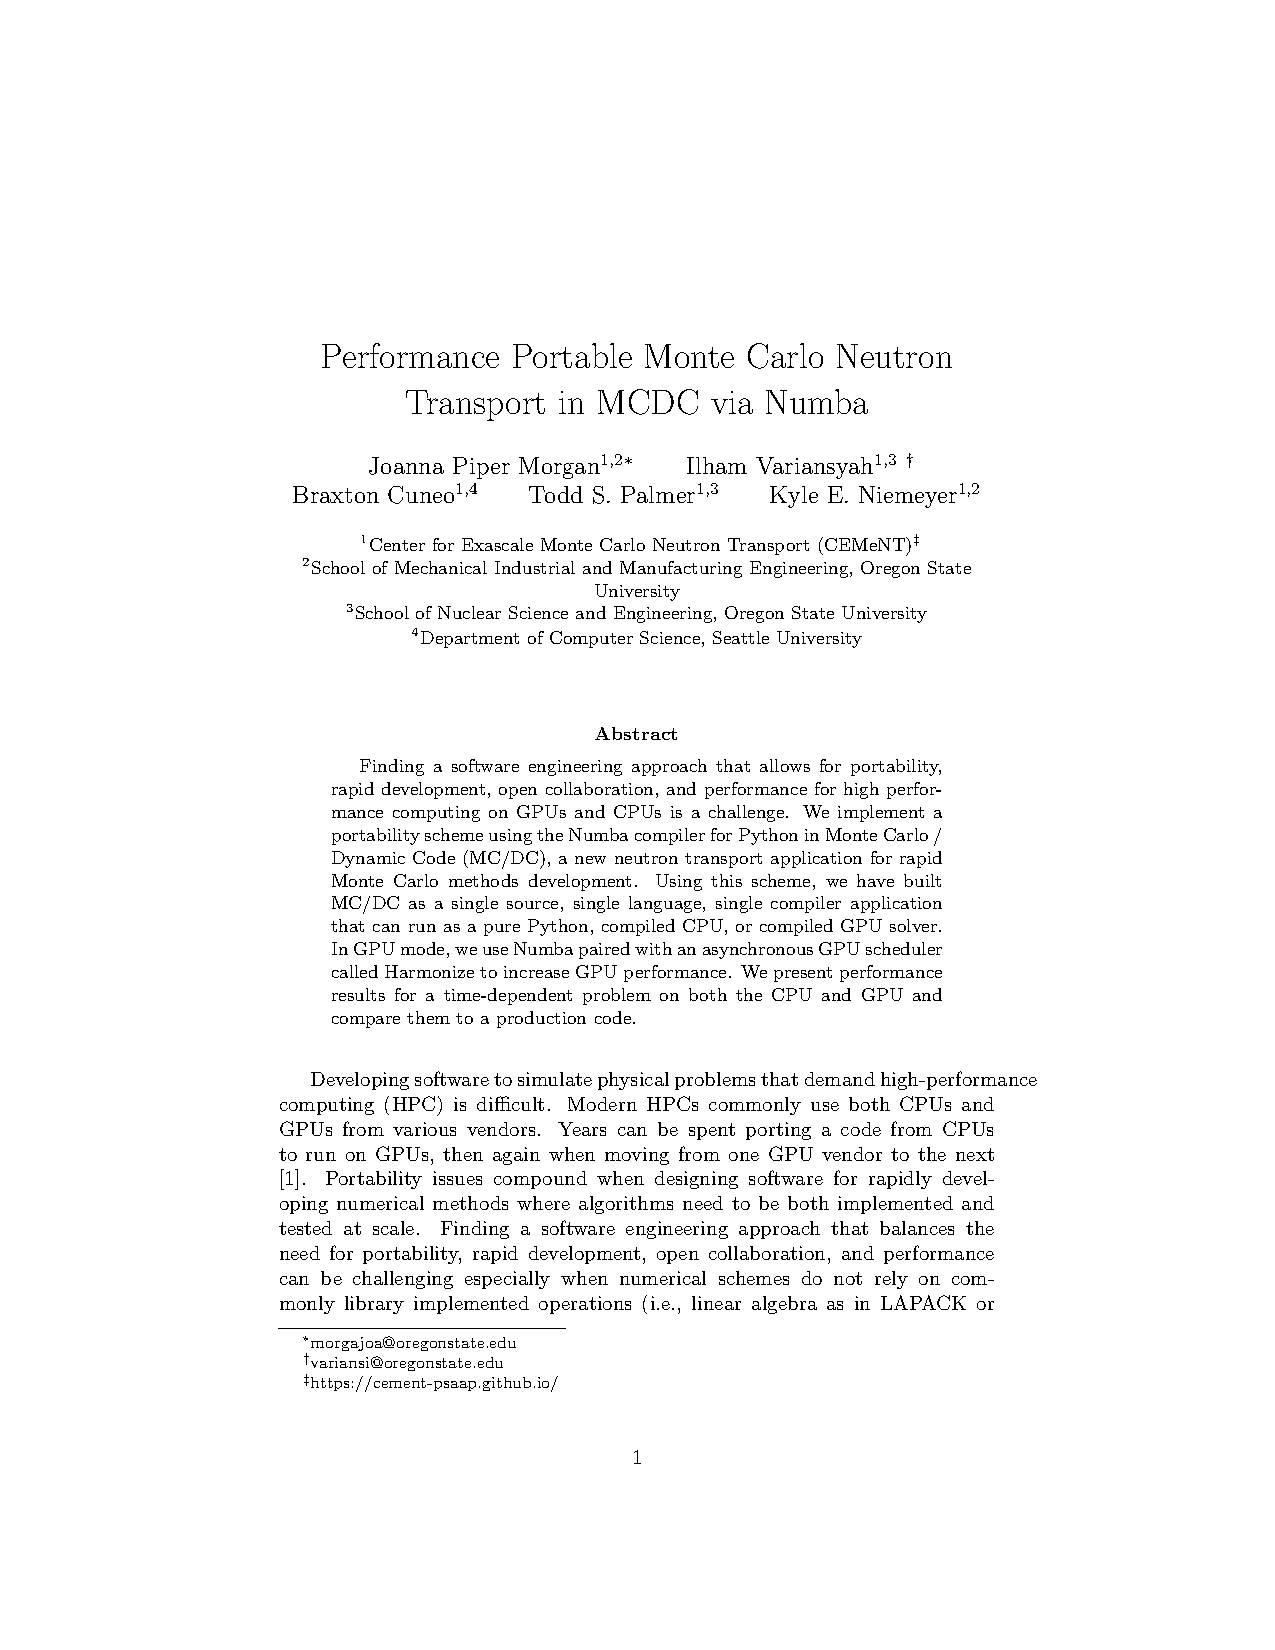
\includepdf[pages=-]{appendix/ana_numba_mcdc.pdf}


\section{Hybrid-Delta Tracking on a Structured Mesh in MCATK}

This work was submitted to, accepted with mino

\begin{itemize}
    \item Travis J. Trahan, PhD
    \item Timothy P. Burke, PhD
    \item Collin J. Josey, PhD
    \item Kyle E. Niemeyer, PhD
\end{itemize}

\label{app:hybridmcatk}
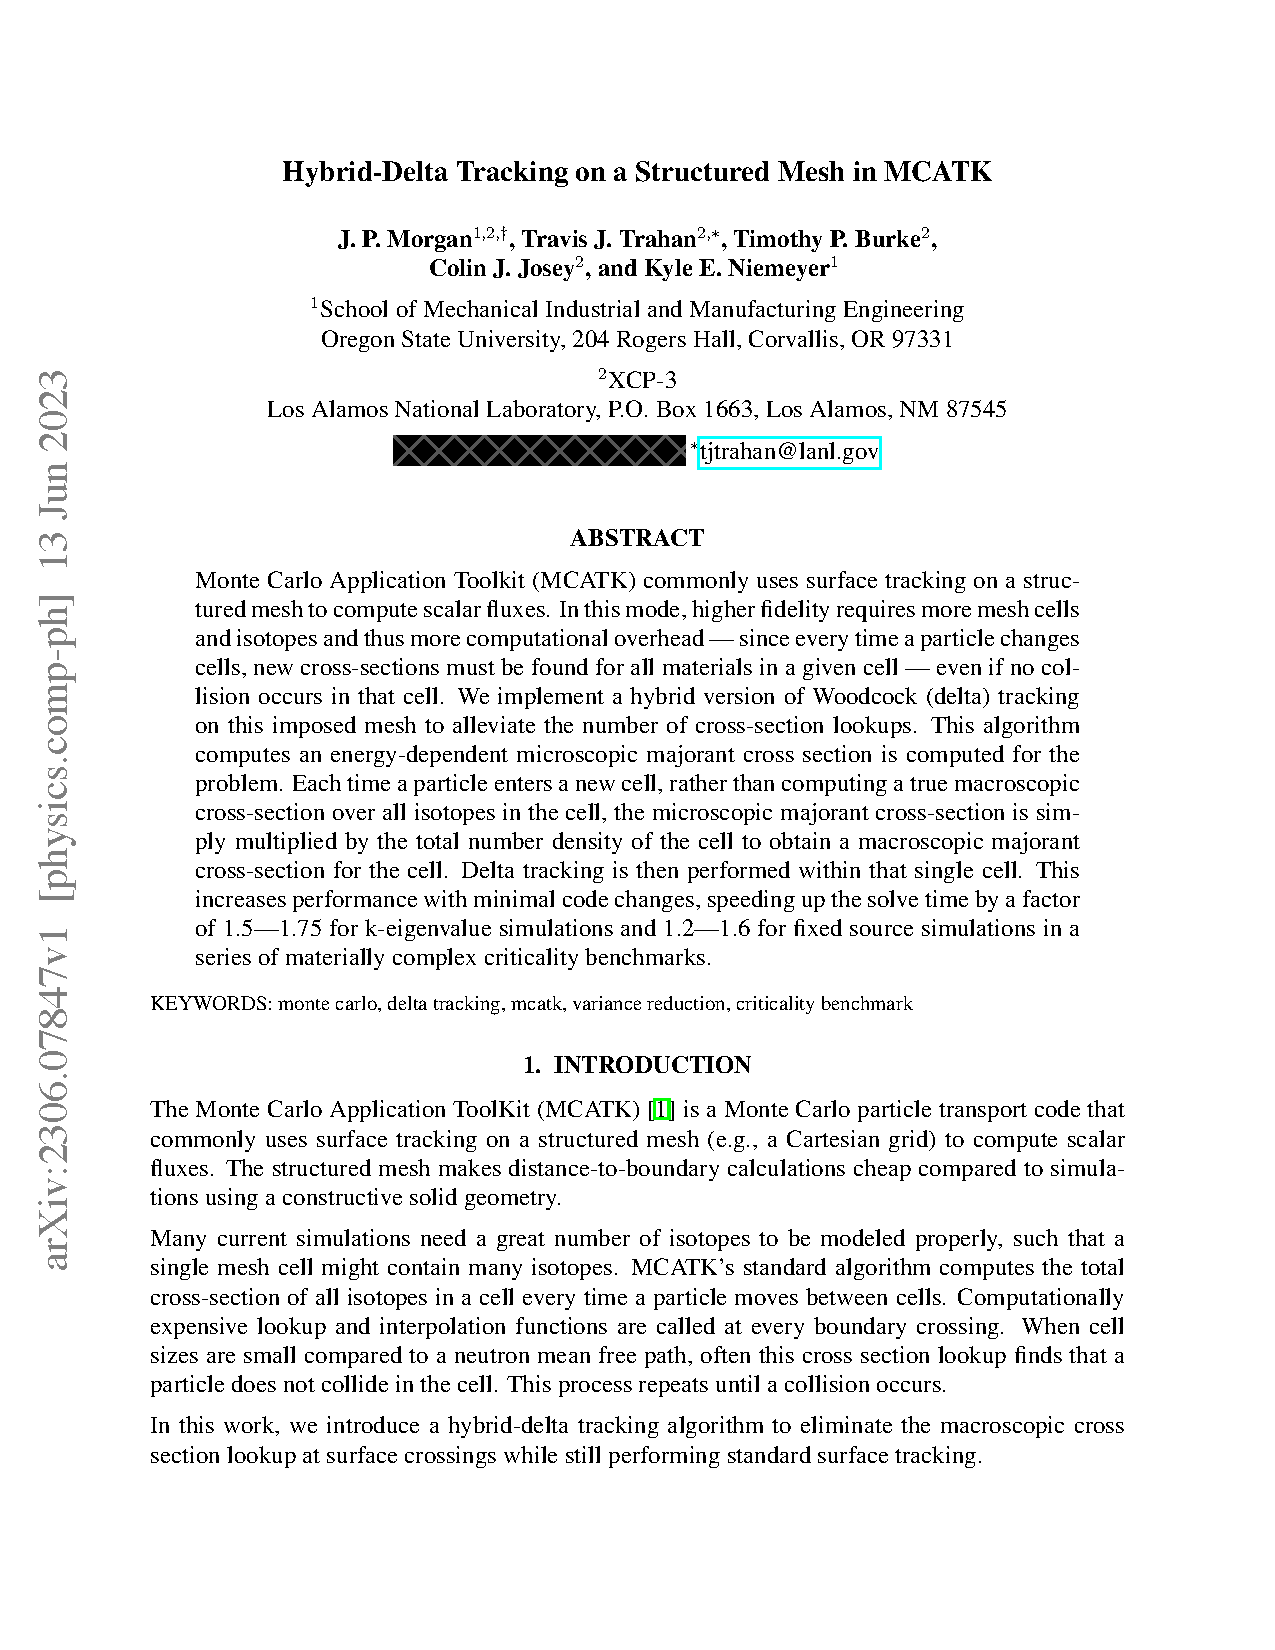
\includepdf[pages=-]{appendix/delta_tracking_mcatk.pdf}

\section{Draft: Therefore paper}
\label{app:therefore}
%\includepdf[pages=-]{ANS2022Clements.pdf}
%\includepdf[pages=-]{OlsonANSWinter2022.pdf}
%\includepdf[pages=-]{journal_draft.pdf}



%\input{Sections/appendixB}
%\input{Sections/appendixC}

%----------------------------------------------------------------------------------------
%	BIBLIOGRAPHY
%----------------------------------------------------------------------------------------

\addtocontents{toc}{\vspace{2em}} % Add a gap in the Contents, for aesthetics
\unnumberedchapter{Bibliography} % Title of the unnumbered chapter
\bibliography{Preamble/Thesis_bibliography} % The references information are stored in the file named "Thesis_bibliography.bib"


\end{document}  